\documentclass[journal]{new-aiaa}
%DIF LATEXDIFF DIFFERENCE FILE


%DIF 2a2
 %DIF > 
%DIF -------
\usepackage{bm}
\usepackage{float}
\usepackage{setspace}



%DIF 7d8
%DIF < \usepackage[utf8]{inputenc}
%DIF -------

%DIF 9a9-10
\usepackage[utf8]{inputenc} %DIF > 
\usepackage[usenames, dvipsnames]{color} %DIF > 
%DIF -------
\usepackage{graphicx}
\usepackage{amsmath}
\usepackage[version=4]{mhchem}
\usepackage{siunitx}
\usepackage{longtable,tabularx}
%DIF 14a16
 %DIF > 
%DIF -------
\setlength\LTleft{0pt} 
%\doublespacing
%\def\bibsection{\section*{References}}

\newcommand{\FirstStageAltConstq}{24.4}
\newcommand{\FirstStageAltFifty}{25.0}
\newcommand{\FirstStageAltFortyFive}{25.6}
\newcommand{\FirstStageAltFiftyFive}{24.0}
\newcommand{\FirstStageAltHighDrag}{25.3}


%\newcommand{\FirstStagemConstq}{17655}
%\newcommand{\FirstStagemFifty}{17792}
%\newcommand{\FirstStagemFortyFive}{17890}
%\newcommand{\FirstStagemFiftyFive}{17495}
%\newcommand{\FirstStagemHighDrag}{17715}

\newcommand{\FirstStagesmfConstq}{.0737}
\newcommand{\FirstStagesmfFifty}{.0732}
\newcommand{\FirstStagesmfFortyFive}{.0728}
\newcommand{\FirstStagesmfFiftyFive}{.0744}
\newcommand{\FirstStagesmfHighDrag}{.0735}

\newcommand{\FirstStagemincrease}{2.2}

\newcommand{\PayloadImprovement}{8.35\%}
\newcommand{\qDecrease}{20.3\%}
\newcommand{\qVariationPluskg}{$+$6.5kg}
\newcommand{\qVariationMinuskg}{$-$6.0kg}
\newcommand{\qVariationPlus}{$+$3.8\%}
\newcommand{\qVariationMinus}{$-$3.5\%}
\newcommand{\vVariationPlus}{$+$12}
\newcommand{\vVariationMinus}{$-$20}

\newcommand{\PayloadToOrbitConstq}{156.8}
\newcommand{\PayloadToOrbitFiftykPa}{169.9}
\newcommand{\PayloadToOrbitFortyFivekPa}{163.9}
\newcommand{\PayloadToOrbitFiftyFivekPa}{176.4}
\newcommand{\PayloadToOrbitHighDrag}{161.8}

\newcommand{\SeparationAltConstq}{33.17}
\newcommand{\SeparationAltFiftykPa}{34.49}
\newcommand{\SeparationAltFortyFivekPa}{34.46}
\newcommand{\SeparationAltFiftyFivekPa}{34.58}
\newcommand{\SeparationAltHighDrag}{34.29}

\newcommand{\SeparationvConstq}{2905}
\newcommand{\SeparationvFiftykPa}{2881}
\newcommand{\SeparationvFortyFivekPa}{2861}
\newcommand{\SeparationvFiftyFivekPa}{2893}
\newcommand{\SeparationvHighDrag}{2829}

\newcommand{\SeparationAngleConstq}{1.50}
\newcommand{\SeparationAngleFiftykPa}{2.91}
\newcommand{\SeparationAngleFortyFivekPa}{2.31}
\newcommand{\SeparationAngleFiftyFivekPa}{3.39}
\newcommand{\SeparationAngleHighDrag}{2.97}

\newcommand{\SeparationqConstq}{46.3}
\newcommand{\SeparationqFiftykPa}{36.9}
\newcommand{\SeparationqFortyFivekPa}{36.59}
\newcommand{\SeparationqFiftyFivekPa}{36.71}
\newcommand{\SeparationqHighDrag}{36.7}

\newcommand{\SeparationLDConstq}{3.21}
\newcommand{\SeparationLDFiftykPa}{3.24}
\newcommand{\SeparationLDFortyFivekPa}{3.35}
\newcommand{\SeparationLDFiftyFivekPa}{3.34}
\newcommand{\SeparationLDHighDrag}{2.94}

\newcommand{\FlightTimeConstq}{349.1}
\newcommand{\FlightTimeFiftykPa}{357.0}
\newcommand{\FlightTimeFortyFivekPa}{381.8}
\newcommand{\FlightTimeFiftyFivekPa}{326.8}
\newcommand{\FlightTimeHighDrag}{356.9}

%\newcommand{\MaxqConstq}{46.28}
%\newcommand{\MaxqFiftykPa}{X}
%\newcommand{\MaxqFortyFivekPa}{X}
%\newcommand{\MaxqFiftyFivekPa}{X}
%\newcommand{\MaxqHighDrag}{X}

\newcommand{\toverConstq}{65}
\newcommand{\toverFiftykPa}{29}
\newcommand{\toverFortyFivekPa}{25}
\newcommand{\toverFiftyFivekPa}{23}
\newcommand{\toverHighDrag}{27}

\renewcommand{\topfraction}{0.9}

\makeatletter
\newcommand*{\rom}[1]{\expandafter\@slowromancap\romannumeral #1@}
\makeatother
%DIF PREAMBLE EXTENSION ADDED BY LATEXDIFF
%DIF UNDERLINE PREAMBLE %DIF PREAMBLE
\RequirePackage[normalem]{ulem} %DIF PREAMBLE
\RequirePackage{color}\definecolor{RED}{rgb}{1,0,0}\definecolor{BLUE}{rgb}{0,0,1} %DIF PREAMBLE
\providecommand{\DIFadd}[1]{{\protect\color{blue}\uwave{#1}}} %DIF PREAMBLE
\providecommand{\DIFdel}[1]{{\protect\color{red}\sout{#1}}}                      %DIF PREAMBLE
%DIF SAFE PREAMBLE %DIF PREAMBLE
\providecommand{\DIFaddbegin}{} %DIF PREAMBLE
\providecommand{\DIFaddend}{} %DIF PREAMBLE
\providecommand{\DIFdelbegin}{} %DIF PREAMBLE
\providecommand{\DIFdelend}{} %DIF PREAMBLE
%DIF FLOATSAFE PREAMBLE %DIF PREAMBLE
\providecommand{\DIFaddFL}[1]{\DIFadd{#1}} %DIF PREAMBLE
\providecommand{\DIFdelFL}[1]{\DIFdel{#1}} %DIF PREAMBLE
\providecommand{\DIFaddbeginFL}{} %DIF PREAMBLE
\providecommand{\DIFaddendFL}{} %DIF PREAMBLE
\providecommand{\DIFdelbeginFL}{} %DIF PREAMBLE
\providecommand{\DIFdelendFL}{} %DIF PREAMBLE
\newcommand{\DIFscaledelfig}{0.5}
%DIF HIGHLIGHTGRAPHICS PREAMBLE %DIF PREAMBLE
\RequirePackage{settobox} %DIF PREAMBLE
\RequirePackage{letltxmacro} %DIF PREAMBLE
\newsavebox{\DIFdelgraphicsbox} %DIF PREAMBLE
\newlength{\DIFdelgraphicswidth} %DIF PREAMBLE
\newlength{\DIFdelgraphicsheight} %DIF PREAMBLE
% store original definition of \includegraphics %DIF PREAMBLE
\LetLtxMacro{\DIFOincludegraphics}{\includegraphics} %DIF PREAMBLE
\newcommand{\DIFaddincludegraphics}[2][]{{\color{blue}\fbox{\DIFOincludegraphics[#1]{#2}}}} %DIF PREAMBLE
\newcommand{\DIFdelincludegraphics}[2][]{% %DIF PREAMBLE
\sbox{\DIFdelgraphicsbox}{\DIFOincludegraphics[#1]{#2}}% %DIF PREAMBLE
\settoboxwidth{\DIFdelgraphicswidth}{\DIFdelgraphicsbox} %DIF PREAMBLE
\settoboxtotalheight{\DIFdelgraphicsheight}{\DIFdelgraphicsbox} %DIF PREAMBLE
\scalebox{\DIFscaledelfig}{% %DIF PREAMBLE
\parbox[b]{\DIFdelgraphicswidth}{\usebox{\DIFdelgraphicsbox}\\[-\baselineskip] \rule{\DIFdelgraphicswidth}{0em}}\llap{\resizebox{\DIFdelgraphicswidth}{\DIFdelgraphicsheight}{% %DIF PREAMBLE
\setlength{\unitlength}{\DIFdelgraphicswidth}% %DIF PREAMBLE
\begin{picture}(1,1)% %DIF PREAMBLE
\thicklines\linethickness{2pt} %DIF PREAMBLE
{\color[rgb]{1,0,0}\put(0,0){\framebox(1,1){}}}% %DIF PREAMBLE
{\color[rgb]{1,0,0}\put(0,0){\line( 1,1){1}}}% %DIF PREAMBLE
{\color[rgb]{1,0,0}\put(0,1){\line(1,-1){1}}}% %DIF PREAMBLE
\end{picture}% %DIF PREAMBLE
}\hspace*{3pt}}} %DIF PREAMBLE
} %DIF PREAMBLE
\LetLtxMacro{\DIFOaddbegin}{\DIFaddbegin} %DIF PREAMBLE
\LetLtxMacro{\DIFOaddend}{\DIFaddend} %DIF PREAMBLE
\LetLtxMacro{\DIFOdelbegin}{\DIFdelbegin} %DIF PREAMBLE
\LetLtxMacro{\DIFOdelend}{\DIFdelend} %DIF PREAMBLE
\DeclareRobustCommand{\DIFaddbegin}{\DIFOaddbegin \let\includegraphics\DIFaddincludegraphics} %DIF PREAMBLE
\DeclareRobustCommand{\DIFaddend}{\DIFOaddend \let\includegraphics\DIFOincludegraphics} %DIF PREAMBLE
\DeclareRobustCommand{\DIFdelbegin}{\DIFOdelbegin \let\includegraphics\DIFdelincludegraphics} %DIF PREAMBLE
\DeclareRobustCommand{\DIFdelend}{\DIFOaddend \let\includegraphics\DIFOincludegraphics} %DIF PREAMBLE
\LetLtxMacro{\DIFOaddbeginFL}{\DIFaddbeginFL} %DIF PREAMBLE
\LetLtxMacro{\DIFOaddendFL}{\DIFaddendFL} %DIF PREAMBLE
\LetLtxMacro{\DIFOdelbeginFL}{\DIFdelbeginFL} %DIF PREAMBLE
\LetLtxMacro{\DIFOdelendFL}{\DIFdelendFL} %DIF PREAMBLE
\DeclareRobustCommand{\DIFaddbeginFL}{\DIFOaddbeginFL \let\includegraphics\DIFaddincludegraphics} %DIF PREAMBLE
\DeclareRobustCommand{\DIFaddendFL}{\DIFOaddendFL \let\includegraphics\DIFOincludegraphics} %DIF PREAMBLE
\DeclareRobustCommand{\DIFdelbeginFL}{\DIFOdelbeginFL \let\includegraphics\DIFdelincludegraphics} %DIF PREAMBLE
\DeclareRobustCommand{\DIFdelendFL}{\DIFOaddendFL \let\includegraphics\DIFOincludegraphics} %DIF PREAMBLE
%DIF END PREAMBLE EXTENSION ADDED BY LATEXDIFF

\begin{document}

%----------------------------------------------------------------------------------------
%	TITLE SECTION
%----------------------------------------------------------------------------------------

\title{Trajectory Design of a Rocket-Scramjet-Rocket Multi-Stage Launch System} % Article title




%----------------------------------------------------------------------------------------
 \author{
 	Sholto O. Forbes-Spyratos%
 	\thanks{Ph.D. Candidate, Centre for Hypersonics, School of Mechanical and Mining Engineering. Member AIAA.}
 	\ ,  Michael P. Kearney
 	\thanks{Lecturer, School of Mechanical and Mining Engineering.}
 	\ ,  Michael K. Smart
 	\thanks{Professor, Centre for Hypersonics, School of Mechanical and Mining Engineering. Senior Member AIAA.}
 	\ and   Ingo H. Jahn
 	\thanks{Lecturer, Centre for Hypersonics, School of Mechanical and Mining Engineering. Member AIAA.}
 	\\
 	{\normalsize\itshape
 		The University of Queensland, Queensland, Australia, 4072}\\
 }



\maketitle

\begin{abstract}

The integration of a reusable scramjet vehicle as \DIFdelbegin \DIFdel{one of the stages of }\DIFdelend \DIFaddbegin \DIFadd{\textcolor{red}{the second} stage of }\DIFaddend a multi-stage space launch system has the potential to reduce the cost of small payload orbital launches. 
This paper determines the maximum payload to orbit trajectory of a multi-stage rocket-scramjet-rocket system. This trajectory is calculated by formulating the problem as an optimal control problem, then solving it using the pseudospectral method. 
Using this method, it is determined that the optimal trajectory for the scramjet stage involves an initial decrease in dynamic pressure, followed by constant dynamic pressure flight, and finally a pull-up manoeuvre. This optimal trajectory results in a \PayloadImprovement\ improvement in payload mass to orbit when compared to a constant dynamic pressure trajectory with minimum pull-up. 
Furthermore, the optimal pull-up manoeuvre decreases the maximum dynamic pressure experienced by the final rocket stage by \qDecrease. 
The sensitivity of the trajectory is tested by varying the maximum allowable dynamic pressure, and the drag produced by the vehicle. 
A maximum dynamic pressure variation of $\pm$5kPa is shown to produce only a \qVariationPlus\ and \qVariationMinus\ variation in payload mass. A drag increase of 10\% is shown to produce a similar optimal trajectory shape, indicating robustness with variation of vehicle aerodynamics. 


\end{abstract}


\section*{Nomenclature}
\noindent
\begin{tabular}{p{1.2cm}p{1cm}p{5cm}}
	 $I_{sp}$ & $=$ & Specific Impulse (s)\\ 
	\end{tabular} 
	  	\begin{tabular}{p{1.2cm}p{1cm}p{5cm}}
	  $t$ & $=$ & Time \DIFaddbegin \DIFadd{\textcolor{red}{(s)}}\DIFaddend \\
	  	\end{tabular} 
	  	\begin{tabular}{p{1.2cm}p{1cm}p{5cm}}
	  $\textbf{x}$& $=$ & \DIFdelbegin \DIFdel{Primal Variables}\DIFdelend \DIFaddbegin \DIFadd{\textcolor{red}{State Variable}s}\DIFaddend \\
	  	\end{tabular} 
	  	\begin{tabular}{p{1.2cm}p{1cm}p{5cm}}
	  $\textbf{u}$& $=$ & Control Variables\\
	  	\end{tabular} 
	  	\begin{tabular}{p{1.2cm}p{1cm}p{5cm}}
	  $q$ & $=$ & Dynamic Pressure (Pa)\\
	  	\end{tabular} 
  		\begin{tabular}{p{1.2cm}p{1cm}p{5cm}}
  		$\psi$ \DIFdelbegin \DIFdel{, }\DIFdelend \DIFaddbegin & \DIFadd{$=$ }& \DIFadd{\textcolor{red}{Equality Constraint Functional}}\\
  	\end{tabular}
  	\begin{tabular}{p{1.2cm}p{1cm}p{5cm}}
  	\DIFaddend $\lambda$ \DIFdelbegin \DIFdel{, }\DIFdelend \DIFaddbegin & \DIFadd{$=$ }& \DIFadd{\textcolor{red}{Inequality Constraint Functional}}\\
  \end{tabular}
	\begin{tabular}{p{1.2cm}p{1cm}p{5cm}}
	 \DIFaddend $M$ \DIFdelbegin \DIFdel{, }\DIFdelend \DIFaddbegin & \DIFadd{$=$ }& \DIFadd{\textcolor{red}{End Point Cost Functional}}\\
\end{tabular}
	\begin{tabular}{p{1.2cm}p{1cm}p{5cm}}
	 \DIFaddend $P$ & $=$ & \DIFdelbegin \DIFdel{Functions}\DIFdelend \DIFaddbegin \DIFadd{\textcolor{red}{Integrated Cost Functional}}\DIFaddend \\
\end{tabular}
	  	\begin{tabular}{p{1.2cm}p{1cm}p{5cm}}
	  $C$ & $=$ & Cost \DIFdelbegin \DIFdel{Function}\DIFdelend \DIFaddbegin \DIFadd{Functional}\DIFaddend \\
	  	\end{tabular} 
	  	\begin{tabular}{p{1.2cm}p{1cm}p{5cm}}
	  $F$ & $=$ & Force (N)\\
	  	\end{tabular} 
	  	\begin{tabular}{p{1.2cm}p{1cm}p{5cm}}
	  $\rho$ & $=$ & Density (kg/m$^2$)\\
	  	\end{tabular} 
	  			\begin{tabular}{p{1.2cm}p{1cm}p{5cm}}
	  				$D$ & $=$ & Drag \DIFaddbegin \DIFadd{\textcolor{red}{(N)}}\DIFaddend \\
	  			\end{tabular} 
	  			\begin{tabular}{p{1.2cm}p{1cm}p{5cm}}
	  				$L$ & $=$ & Lift \DIFaddbegin \DIFadd{\textcolor{red}{(N)}}\DIFaddend \\
	  			\end{tabular} 
	  	\begin{tabular}{p{1.2cm}p{1cm}p{5cm}}
	  $C_L,C_D$ & $=$ & Aerodynamic Coefficients\\
	  	\end{tabular} 
  	\begin{tabular}{p{1.2cm}p{1cm}p{5cm}}
  		\DIFaddbegin \DIFadd{$\textcolor{red}{\xi}$ }& \DIFadd{$=$ }& \DIFadd{Longitude (rad)}\\
  	\end{tabular} 
  \begin{tabular}{p{1.2cm}p{1cm}p{5cm}}
  	\DIFadd{$\textcolor{red}{\phi}$ }& \DIFadd{$=$ }& \DIFadd{Latitude (rad)}\\
  \end{tabular} 
\begin{tabular}{p{1.2cm}p{1cm}p{5cm}}
	\DIFadd{$\textcolor{red}{\zeta}$ }& \DIFadd{$=$ }& \DIFadd{Heading Angle (rad)}\\
\end{tabular} 
	  	\begin{tabular}{p{1.2cm}p{1cm}p{5cm}}
	  \DIFaddend $v$ & $=$ & Velocity (m/s)\\
	  	\end{tabular} 
	  	\begin{tabular}{p{1.2cm}p{1cm}p{5cm}}
	  $A$ & $=$ & Reference Area (m$^2$)\\
	  	\end{tabular} 
	  	\begin{tabular}{p{1.2cm}p{1cm}p{5cm}}
	  		$g_0$ & $=$ & Gravitational Acceleration at Earth's Surface (m/s$^2$)\\
	  	\end{tabular} 
	  	\begin{tabular}{p{1.2cm}p{1cm}p{5cm}}

	
	$r$ & $=$ & Radius from Earth Centre (m)\\
		\end{tabular} 
		\begin{tabular}{p{1.2cm}p{1cm}p{5cm}}
	  $\gamma$ & $=$ & \DIFdelbegin \DIFdel{Trajectory Angle }\DIFdelend \DIFaddbegin \DIFadd{\textcolor{red}{flight path angle} }\DIFaddend (rad)\\
	  	\end{tabular} 
	  	\begin{tabular}{p{1.2cm}p{1cm}p{5cm}}
	  $\omega$ & $=$ & Angular Velocity (rad/s)\\
	  	\end{tabular} 
	  	\begin{tabular}{p{1.2cm}p{1cm}p{5cm}}
	  $a$ & $=$ & Acceleration (m/s$^2$)\\
	  	\end{tabular} 
	  	\begin{tabular}{p{1.2cm}p{1cm}p{5cm}}
	  $m$ & $=$ & Mass (kg)\\
	  	\end{tabular} 
	  	\begin{tabular}{p{1.2cm}p{1cm}p{5cm}}
	  $T$ & $=$ & Thrust (N)\\
	  	\end{tabular} 
	  	\begin{tabular}{p{1.2cm}p{1cm}p{5cm}}
	  $w_{cap}$ & $=$ & Capture Width\\
	  	\end{tabular} 
	  	\begin{tabular}{p{1.2cm}p{1cm}p{5cm}}
	  		$\alpha$ & $=$ & Angle of Attack (rad)\\
	  	\end{tabular} 	
	  	\DIFdelbegin %DIFDELCMD < \begin{tabular}{p{1.2cm}p{1cm}p{5cm}}
%DIFDELCMD < 	  		%%%
\DIFdel{$\phi$ }%DIFDELCMD < & %%%
\DIFdel{$=$ }%DIFDELCMD < & %%%
\DIFdel{Equivalence Ratio}%DIFDELCMD < \\
%DIFDELCMD < 	  	\end{tabular} 
%DIFDELCMD < 	  	%%%
\DIFdelend \newline  	
	  	\begin{tabular}{p{5.2cm}p{1cm}p{5cm}}


\textit{Subscripts} \\
\end{tabular} 
\newline
\begin{tabular}{p{1.2cm}p{1cm}p{5cm}}
	$E$ & $=$ & Earth\\

\end{tabular} 
\begin{tabular}{p{1.2cm}p{1cm}p{5cm}}
$1$ & $=$ & $1^{st}$ Stage Rocket\\
\end{tabular} 
\begin{tabular}{p{1.2cm}p{1cm}p{5cm}}
	$2$ & $=$ & $2^{nd}$ Stage Scramjet Vehicle\\
		\end{tabular} 
		\begin{tabular}{p{1.2cm}p{1cm}p{5cm}}
	$3$ & $=$ & $3^{rd}$ Stage Rocket\\
		\end{tabular} 
		\begin{tabular}{p{1.2cm}p{1cm}p{5cm}}
	$\rightarrow$ & = & Stage Transition\\
		\end{tabular} 
				\begin{tabular}{p{1.2cm}p{1cm}p{5cm}}
					$0$ & $=$ & Initial\\
				\end{tabular} 
		\begin{tabular}{p{1.2cm}p{1cm}p{5cm}}
	$f$ & $=$ & Final\\
\end{tabular} 
\begin{tabular}{p{1.2cm}p{1cm}p{5cm}}
	$a,b$ & $=$ & Nominal Stage Numbers\\
\end{tabular} 
\begin{tabular}{p{1.2cm}p{1cm}p{5cm}}
	LOX & $=$ & Liquid Oxygen\\
\end{tabular} 
\begin{tabular}{p{1.2cm}p{1cm}p{5cm}}
	LH2 & $=$ & Liquid Hydrogen\\

\end{tabular} 
\begin{tabular}{p{1.2cm}p{1cm}p{5cm}}
	AoA & $=$ & Angle of Attack\\

\end{tabular} 
\begin{tabular}{p{1.2cm}p{1cm}p{5cm}}
	e & $=$ & Exit\\
\end{tabular} 
\begin{tabular}{p{1.2cm}p{1cm}p{5cm}}
	$SL$ & $=$ & Sea Level\\
\end{tabular} 
\begin{tabular}{p{1.2cm}p{1cm}p{5cm}}
	$atm$ & $=$ & Atmospheric\\

\end{tabular} 
\begin{tabular}{p{1.2cm}p{1cm}p{5cm}}
	$vac$ & $=$ & Vacuum\\

\end{tabular} 
\begin{tabular}{p{1.2cm}p{1cm}p{5cm}}
	$LEO$ & $=$ & Low Earth Orbit\\

\end{tabular} 
\newpage
\section{Introduction}






Currently, most small satellites co-manifest with a larger payload, leaving their launch schedule and trajectory at the mercy of the major payload. The  increasing demand for small satellite launches\cite{Faa&Ast&Comstac2015} is driving the development of cheap and efficient launch systems for independent launches of small satellites into tailored orbits, on a fast schedule. 
A multi-stage launch system incorporating a scramjet second stage has been proposed as a dedicated small satellite launch vehicle\cite{Smart2009a}. 
Scramjets (supersonic combustion ramjets) are airbreathing engines that operate over Mach numbers in the hypersonic  range\cite{HeiserWilliamPratt1994}. 
Scramjet engines are a primary candidate for powering the next generation of small payload launch vehicles, producing higher specific impulse ($I_{sp}$)  than rockets within their operating range. Other benefits of scramjets include increased flexibility of launch windows and an increased range of mission capabilities\cite{Flaherty2010}. 
Scramjets can accelerate a launch vehicle without the need to carry oxidiser on board, providing mass savings compared to rocket-powered vehicles. 
 The reduction of mass carried within the vehicle fuselage enables the integration of avionics and landing gear, allowing for the design of a reusable vehicle in the style of conventional aerospace vehicles. 
However, a \DIFdelbegin \DIFdel{launch system must contain three }\DIFdelend \DIFaddbegin \DIFadd{\textcolor{red}{scramjet incorporating} launch system \textcolor{red}{requires two rocket} }\DIFaddend stages, a first stage rocket capable of accelerating the scramjet vehicle to its operating speed and a final rocket stage for placing the payload in orbit. 


This paper presents a trajectory designed using optimal control methods for a rocket-scramjet-rocket, small satellite launch system proposed by the Centre for Hypersonics at The University of Queensland\DIFdelbegin \DIFdel{\mbox{%DIFAUXCMD
\cite{Preller2017}}%DIFAUXCMD
}\DIFdelend \DIFaddbegin \DIFadd{\mbox{%DIFAUXCMD
\cite{Preller2017b}}%DIFAUXCMD
, \textcolor{red}{incorporating the SPARTAN scramjet accelerator}}\DIFaddend . 
The trajectory profile of this rocket-scramjet-rocket system \DIFdelbegin \DIFdel{, which utilises the SPARTAN scramjet accelerator, }\DIFdelend has previously been designed around the scramjet stage flying a constant dynamic pressure trajectory\DIFdelbegin \DIFdel{\mbox{%DIFAUXCMD
\cite{Preller2017}}%DIFAUXCMD
}\DIFdelend \DIFaddbegin \DIFadd{\mbox{%DIFAUXCMD
\cite{Preller2017b}}%DIFAUXCMD
}\DIFaddend , in-line with similar multi-stage vehicles\cite{Kimura1999,Olds1998}.
 A constant dynamic pressure trajectory follows the maximum dynamic pressure that the scramjet-powered vehicle is able to withstand structurally, ensuring maximum thrust production from the scramjet engines. However, flying a maximum dynamic pressure trajectory also results in the release of the third stage rocket into a high dynamic pressure, at low \DIFdelbegin \DIFdel{trajectory angle}\DIFdelend \DIFaddbegin \DIFadd{\textcolor{red}{flight path angle}}\DIFaddend . 


 Previously, when flying a constant dynamic pressure scramjet-stage trajectory, the Pratt \& Whitney RL-10A-3A pump-fed engine was used as the propulsion system for the third stage rocket\DIFdelbegin \DIFdel{\mbox{%DIFAUXCMD
\cite{Preller2017}}%DIFAUXCMD
}\DIFdelend \DIFaddbegin \DIFadd{\mbox{%DIFAUXCMD
\cite{Preller2017b}}%DIFAUXCMD
}\DIFaddend . This study instead utilises a modified SpaceX Kestrel engine\cite{Vehicle2008}. This is more cost efficient than the RL-10-3A, with the trade-off of lower thrust and efficiency. Due to the reduced thrust, the Kestrel powered third stage is unable to reach orbit if released from a near horizontal flight at maximum dynamic pressure. Instead a minimal pull-up is required to release the third stage at lower dynamic pressure.

 A trajectory with the minimum \DIFdelbegin \DIFdel{allowable }\DIFdelend \DIFaddbegin \DIFadd{\textcolor{red}{required} }\DIFaddend pull-up produces maximum acceleration from the scramjet stage, by maximising the dynamic pressure during flight. However, a minimum pull-up trajectory may not be optimal for the overall multi-stage system. 
 For example, a minimum pull-up trajectory may still release the final stage into a high dynamic pressure environment, at a potentially suboptimal \DIFdelbegin \DIFdel{trajectory angle}\DIFdelend \DIFaddbegin \DIFadd{\textcolor{red}{flight path angle}}\DIFaddend . This release point may result in suboptimal performance of the final stage rocket  and the inclusion of unnecessary design constraints. 
 A larger pull-up may produce an overall favourable trade-off, by allowing for the scramjet stage to be used to increase the altitude and flight path angle of the launch vehicle, enabling the final stage rocket to operate with reduced drag.
 However, as the altitude increases, the thrust of the airbreathing engine is reduced, due to a lower mass flow rate into the engine. 


  
 In previous studies, \DIFdelbegin \DIFdel{optimal control methods have been used to analyse the trajectories of launch vehicles utilising rocket and airbreathing propulsion within a single stage\mbox{%DIFAUXCMD
\cite{Powell1991,Lu1993,Trefny1999}}%DIFAUXCMD
. The optimised trajectories for these single stage vehicles show flight at maximum dynamic pressure for the majority of airbreathing operation}\DIFdelend \DIFaddbegin \DIFadd{\textcolor{red}{the optimised trajectories for launch vehicles utilising rocket and airbreathing propulsion within a single stage have been shown to exhibit flight at maximum dynamic pressure for the majority of airbreathing operation}}\DIFaddend , followed by a pull-up before airbreathing engine cut-off\DIFdelbegin \DIFdel{\mbox{%DIFAUXCMD
\cite{Powell1991,Lu1993,Trefny1999}}%DIFAUXCMD
}\DIFdelend \DIFaddbegin \DIFadd{\textcolor{red}{\cite{Powell1991,Lu1993,Trefny1999,Roche2000,Pescetelli2012,Young2006,Bradford2000}}}\DIFaddend . 
 A trajectory involving a pull-up has been shown to be the optimal trajectory for vehicles where the rocket engines are not ignited until circularization altitude\cite{Powell1991,Lu1993}\DIFdelbegin \DIFdel{as well as }\DIFdelend \DIFaddbegin \DIFadd{\textcolor{red}{,} }\DIFaddend vehicles where the rocket engine is ignited immediately after airbreathing engine cut-off\DIFdelbegin \DIFdel{\mbox{%DIFAUXCMD
\cite{Trefny1999}}%DIFAUXCMD
}\DIFdelend \DIFaddbegin \DIFadd{\textcolor{red}{\cite{Trefny1999,Roche2000,Pescetelli2012} as well as for vehicles which operate in combined scramjet-rocket mode\cite{Young2006,Bradford2000}}}\DIFaddend .


 For launch systems with airbreathing and rocket propulsion combined within a single stage, an optimised pull-up manoeuvre is a simple trade-off between velocity and altitude. However, for the proposed scramjet-rocket multi-stage system, the scramjet stage and rocket stage are sequential and separate completely.
 The resultant change in mass and aerodynamic characteristics adds to the complexity of the trajectory analysis.
 For a robust multi-stage trajectory design there is a trade-off between: 
 \rom{1}. The high efficiency of the scramjet engines,
\rom{2}. The thrust produced by the scramjet engines, 
\rom{3}. The potential thrust of the rocket engines after separation,
\rom{4}. The energy necessary to increase the altitude of the scramjet stage,
\rom{5}. The aerodynamic efficiency when performing the required direction change.


  A pull-up manoeuvre has previously been identified as having potential advantages for multi-stage airbreathing-rocket systems\cite{Tsuchiya2005,Wilhite1991,Mehta2001}. 
  However, these pull-up manoeuvres were minimum pull-ups \DIFdelbegin \DIFdel{performed in order to decrease the dynamic pressure to the operable limit of the rocket stage}\DIFdelend \DIFaddbegin \DIFadd{\textcolor{red}{imposed by rocket flight constraints}}\DIFaddend \cite{Tsuchiya2005,Wilhite1991}, or were prescribed in a suboptimal trajectory with variation in dynamic pressure\cite{Mehta2001}. 
   The inherent intricacies of a multi-stage, partially-airbreathing system, particularly the complexity of transition between airbreathing and rocket stages, necessitates an investigation into the optimal launch trajectory design. 


   
   

This paper utilises optimal control theory to generate the optimal trajectory path for a rocket-scramjet-rocket multi-stage vehicle.
Optimal control theory allows a trajectory to be optimised in its entirety and has been widely used in aerospace applications for computing trajectories when there is a global objective to be optimised, such as minimum fuel\DIFdelbegin \DIFdel{or maximum payload delivery \mbox{%DIFAUXCMD
\cite{Bedrossian,Josselyn2002,Sekhavat2005}}%DIFAUXCMD
. 
Optimal control is also extremely flexible, as the optimal control problem can be modified easily to investigate a range of trajectory objectives \mbox{%DIFAUXCMD
\cite{Ranieri2005}}%DIFAUXCMD
.
}\DIFdelend \DIFaddbegin \DIFadd{\textcolor{red}{\cite{Bedrossian,Josselyn2002,Yang2017} or maximum crossrange\cite{Rizvi2015,Chai2015,Moshman2014}}. 
\textcolor{red}{Prescribing a trajectory to produce an optimal result, using a defined flight path or targeted controller, requires the optimal trajectory conditions to be known a priori. Optimal control allows for the calculation of a flight path which optimises the end goal, while satisfying all vehicle constraints, from few initial assumptions\cite{Rao2009}}.
}

\DIFaddend Highly nonlinear control problems (such as a complex model of hypersonic flight) necessitate the use of direct methods such as direct single shooting, multiple shooting, or collocation\DIFaddbegin \DIFadd{\mbox{%DIFAUXCMD
\cite{Rao2009}}%DIFAUXCMD
}\DIFaddend .
Direct methods discretise the \DIFaddbegin \DIFadd{\textcolor{red}{trajectory optimisation }}\DIFaddend problem, and solve the nonlinear programming \DIFaddbegin \DIFadd{\textcolor{red}{(NLP)} }\DIFaddend problem that results \DIFdelbegin \DIFdel{\mbox{%DIFAUXCMD
\cite{Fahroo2000}}%DIFAUXCMD
. 
The pseudospectral collocation method of optimal control }\DIFdelend \DIFaddbegin \DIFadd{\textcolor{red}{computationally\cite{Fahroo2000,Stryk1992}. This solution is calculated using an NLP solving technique such as sequential quadratic programming (SQP), which is widely used for trajectory optimisation due to its high efficacy\cite{Rao2009,Boggs2000}. The most powerful methods of optimal control are arguably direct collocation methods, in which the state and control variables are approximated using specified basis functions of splines or polynomials\cite{Rao2009,Fahroo2000,Elganar}. The use of global orthogonal polynomials as basis functions, collocated at nodes obtained from a Gaussian quadrature, is referred to as the pseudospectral method, due to the resultant accuracy of the problem converging spectrally (at an exponential rate) as the number of collocation nodes increases\cite{Rao2009,Garg2009}. The use of the spectral method ensures that higher order terms of the dynamic equations are solved, and facilitates solution with high accuracy, even with relatively few collocation points\cite{Fahroo1999}.}
The pseudospectral method }\DIFaddend is utilised in this study due to its accuracy, efficiency, and radius of convergence when compared to other optimal control techniques\cite{Fahroo2000,Elganar}. \DIFaddbegin \DIFadd{\textcolor{red}{The accuracy and validity of this method has been demonstrated for a variety of aerospace applications\cite{Bedrossian,Huntington2008,Josselyn2002,Yan2007}}. 
}\DIFaddend 


The remainder of the paper is as follows: Section \ref{section:system} presents the design characteristics of all three stages. Section \ref{section:aero} presents the aerodynamic modelling of the system. Section \ref{section:optimisation} presents an overview of the optimal control theory used including the problem definition and a description of the pseudospectral method. Section \ref{section:results} presents optimal trajectory results for all three stages, including results verifying the use of the pseudospectral method, optimal trajectory results for a range of maximum dynamic pressure conditions, and optimal trajectory results with variation in the vehicle's aerodynamic characteristics.

\section{The SPARTAN System} \label{section:system}

The system to be optimised, shown in Figures \ref{fig:NoInternal} and \ref{fig:INTERNALS}, includes a rocket-powered first stage, a scramjet-powered second stage, and a rocket-powered third stage for payload delivery to heliosynchronous orbit. The SPARTAN system\DIFdelbegin \DIFdel{\mbox{%DIFAUXCMD
\cite{Preller2015a,Jazra2013,Preller2017}  }%DIFAUXCMD
}\DIFdelend \DIFaddbegin \DIFadd{\mbox{%DIFAUXCMD
\cite{Preller2015a,Jazra2013,Preller2017b}  }%DIFAUXCMD
}\DIFaddend is utilised in this study as a representative model for future multi-stage access to space systems, incorporating airbreathing second stages. The following section details the design characteristics of all three stages.

\begin{figure}[ht]
	\centering
	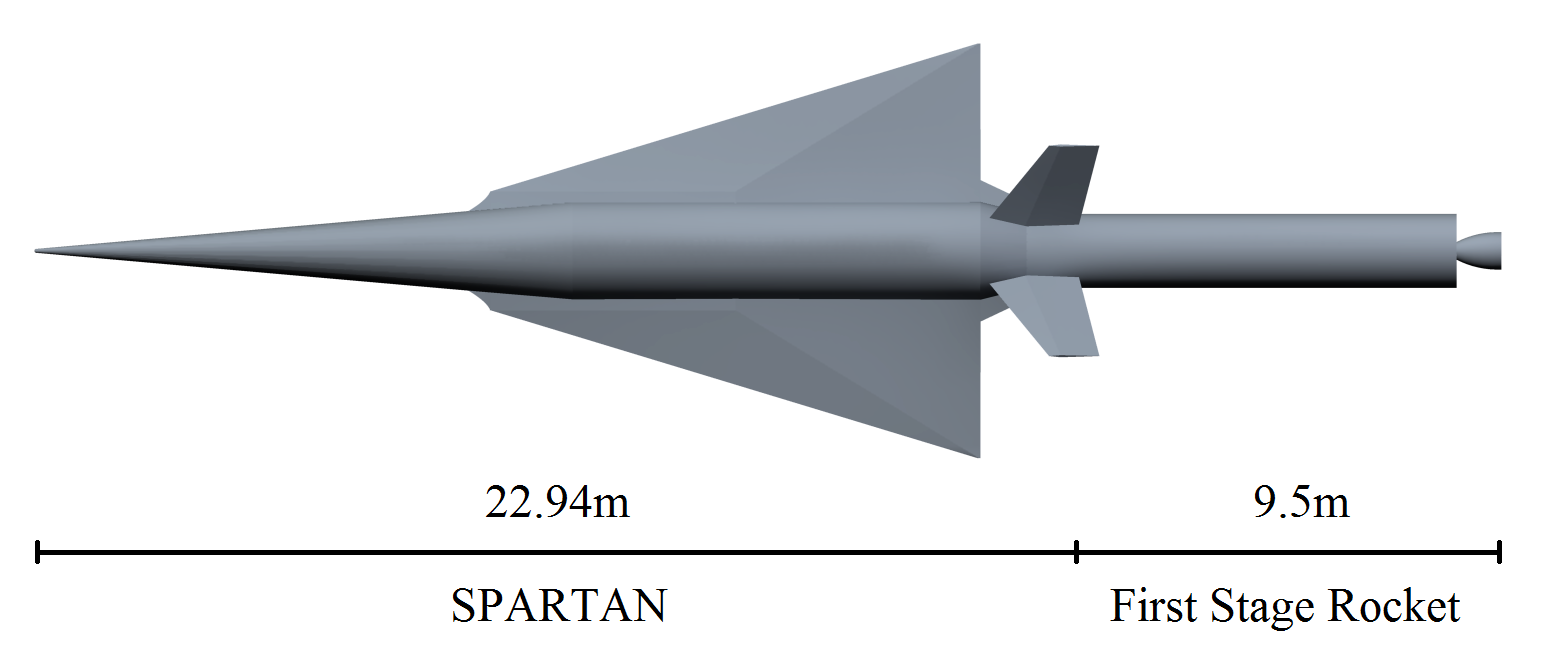
\includegraphics[width=.8\linewidth]{NoInternal}
	\caption{Model of the first stage rocket and scramjet vehicle.}
	\label{fig:NoInternal}
\end{figure}


\begin{figure}[ht]
	\centering
	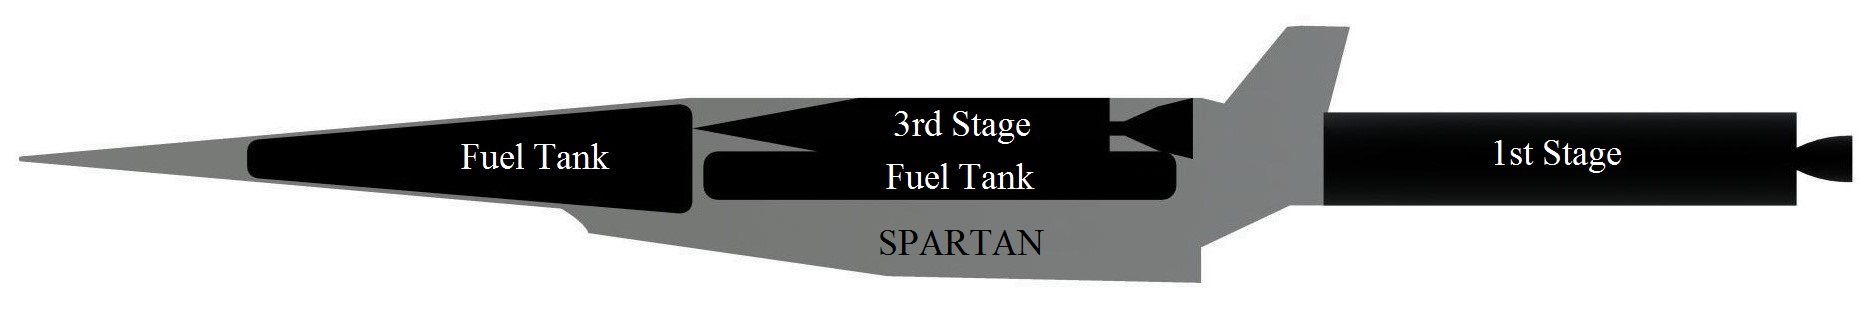
\includegraphics[width=0.8\linewidth]{INTERNALS}
	\caption{Side view of all three stages including internal view.}
	\label{fig:INTERNALS}
\end{figure}

\subsection{The First Stage Rocket}




The first stage rocket is required to deliver the second stage to near horizontal flight at Mach 5.1 flight conditions, after which it is discarded. To achieve this, the first stage rocket is modelled as a Falcon-1e first stage scaled down lengthwise to 9.5m, keeping the original diameter of 1.67m\cite{Vehicle2008}. The first stage is attached to the rear of the scramjet second stage and is powered by a single LOX-kerosene Merlin 1-C engine.  This first stage has a structural mass of 1356kg, determined by scaling of the structural mass of the Falcon-1e. Engine mass is kept constant. The mass of the fuel in the first stage is scaled as part of the optimisation routine, as the dynamics of the vehicle, and its ability to reach a given separation point, are very closely coupled to the available fuel mass. 




\subsection{The Scramjet Accelerator}
The Scramjet-Powered Accelerator for Reusable Technology AdvaNcement (SPARTAN) is a scramjet-powered accelerator under development by the University of Queensland, to be used as the second stage in a scramjet-rocket-powered system for delivering small payloads to heliosynchronous orbit\DIFdelbegin \DIFdel{\mbox{%DIFAUXCMD
\cite{Preller2017}}%DIFAUXCMD
}\DIFdelend \DIFaddbegin \DIFadd{\mbox{%DIFAUXCMD
\cite{Preller2017b}}%DIFAUXCMD
}\DIFaddend . The SPARTAN is designed to be capable of flying back after separation to a designated airfield close to the launch site.  

The SPARTAN has a fuselage diameter of 2.1m and a mass of 9819kg, including the third stage rocket. It has been sized to hold the third stage rocket within the fuselage to reduce aerodynamic drag, as shown in Figure \ref{fig:INTERNALS}. The SPARTAN has three fuel tanks, two cylindrical tanks housed below the third stage rocket, and one conical tank housed in the nose of the vehicle. These tanks have a total volume of 22.0m$^2$, and a total LH2 storage capacity of 1562kg. 
The SPARTAN is powered by four scramjet engines located on the bottom portion of the fuselage, sized to a nominal capture width of 0.65m. These engines are based on the Rectangular-to-Elliptical Shape Transition (REST) scramjet engine design\cite{Suraweera2009} with modified inlets to fit to a conical fuselage via a C-REST inlet configuration\cite{Gollan2010}. Previous studies have indicated that using the SPARTAN as part of a three stage access to space system can produce payload mass fractions that compare favourably with similarly sized rocket systems\DIFdelbegin \DIFdel{\mbox{%DIFAUXCMD
\cite{Preller2015a,Preller2017}}%DIFAUXCMD
}\DIFdelend \DIFaddbegin \DIFadd{\mbox{%DIFAUXCMD
\cite{Preller2015a,Preller2017b}}%DIFAUXCMD
}\DIFaddend . 


\subsection{The Third Stage Rocket}\label{section:rocket}
\begin{figure}[ht]
	\centering
	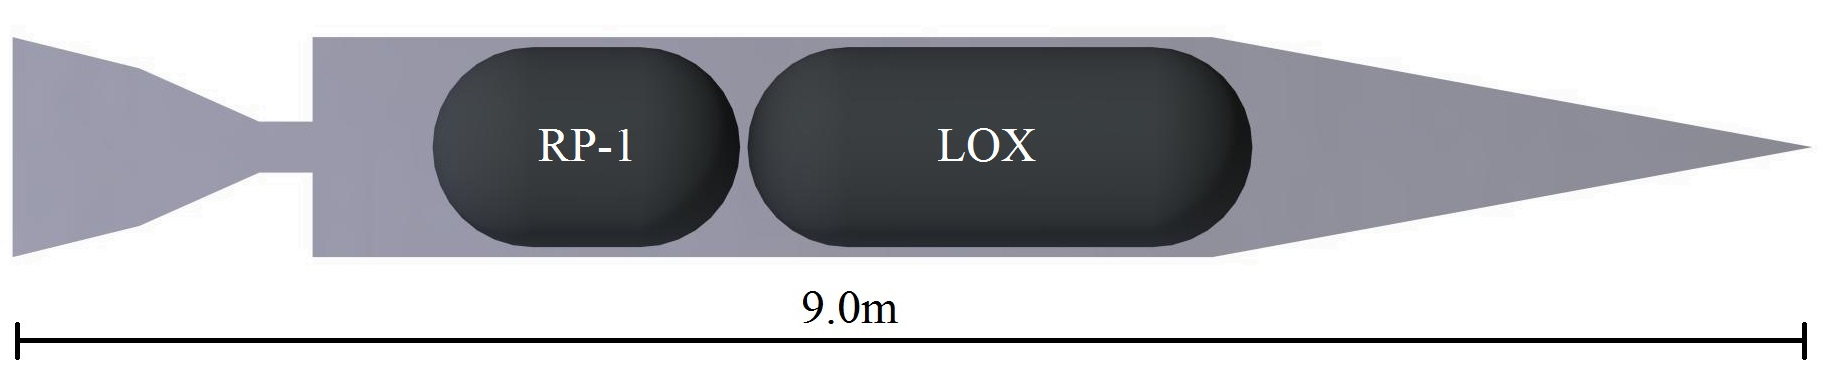
\includegraphics[width=0.6\linewidth]{3rdStage}
	\caption{Schematic of the third stage rocket.}
	\label{fig:ThirdStage}
\end{figure}

The third stage rocket is initially housed within the SPARTAN fuselage, as shown in Figure \ref{fig:INTERNALS}. After separation from the SPARTAN, the third stage rocket initiates a burn, and performs an altitude increasing manoeuvre. 
At the end of the initial burn, the third stage rocket is allowed to coast until reaching apogee, at which point it must have an altitude of at least 100km to ensure that the rocket is in an exoatmospheric orbit. The orbit is circularised using a further short burn, after which the payload delivery to heliosynchronous orbit is completed using a Hohmann transfer. The payload-to-orbit is determined by calculating the mass of the vehicle at the end of the Hohmann transfer. The structural mass is removed, and the remaining mass is taken to be the payload-to-orbit capability of the vehicle. 

\DIFdelbegin \DIFdel{To achieve this, the }\DIFdelend \DIFaddbegin \DIFadd{The }\DIFaddend third stage rocket (Figure \ref{fig:ThirdStage}) has a total length of 9m, diameter of 1.1m and a total initial mass of 3300kg. It is modelled to be powered by a modified SpaceX LOX-kerosene Kestrel engine\cite{Vehicle2008}, weighing 52kg. Previous studies used a LOX-LH2 upper stage based on the RL-10-3A engine\DIFdelbegin \DIFdel{\mbox{%DIFAUXCMD
\cite{Preller2017}}%DIFAUXCMD
}\DIFdelend \DIFaddbegin \DIFadd{\mbox{%DIFAUXCMD
\cite{Preller2017b}}%DIFAUXCMD
}\DIFaddend . In this study the pressure-fed Kestrel engine is used rather than the pump-fed RL-10-3A to reduce the cost of the disposable third stage rocket. The third stage has a structural mass of 285.7kg, equivalent to a structural mass fraction of 0.09 (calculated without heat shield), similar to the Falcon-1e second stage\cite{Vehicle2008}. The in-atmosphere, high dynamic pressure separation of the rocket stage requires the use of a heat shield that envelopes the rocket stage. The heat shield is constructed from a Tungsten nose piece, a Carbon-Carbon cone, and a phenolic cork cylinder. The heat shield weighs 130.9kg in total, and is discarded when the rocket reaches a dynamic pressure of 10Pa (atmospheric heating is assumed to be negligible at this point)\DIFdelbegin \DIFdel{\mbox{%DIFAUXCMD
\cite{Preller2015a,Preller2017}}%DIFAUXCMD
}\DIFdelend \DIFaddbegin \DIFadd{\mbox{%DIFAUXCMD
\cite{Preller2015a,Preller2017b}}%DIFAUXCMD
}\DIFaddend . 


\section{Aerodynamics, Propulsion and Dynamic Modelling}\label{section:aero}

Multiple analysis tools are used to model the aerodynamics and propulsion of the stages of the SPARTAN system. These have been chosen based on appropriateness for the design and Mach number regime of each stage. 

\subsection{Aerodynamics}

An aerodynamic database of the first stage stack is generated using CART3D\cite{CART3D}, a high-fidelity inviscid analysis CFD package with adjoint based mesh refinement. The CART3D package uses a Cartesian cut-cell approach\DIFdelbegin \DIFdel{\mbox{%DIFAUXCMD
\cite{Aftosmis1997} }%DIFAUXCMD
}\DIFdelend \DIFaddbegin \DIFadd{\mbox{%DIFAUXCMD
\cite{Aftosmis1998} }%DIFAUXCMD
}\DIFaddend resulting in a mesh of cubes everywhere except at body-intersecting cells. CART3D is used to analyse the first stage stack due to its applicability over a wide range of Mach numbers. CART3D has been used successfully in a variety of aerospace applications including hypersonic launch systems\cite{Mehta2015} and has shown \DIFdelbegin \DIFdel{good }\DIFdelend \DIFaddbegin \DIFadd{\textcolor{red}{fair} }\DIFaddend agreement when compared to experimental results \DIFdelbegin \DIFdel{\mbox{%DIFAUXCMD
\cite{Aftosmis2011}}%DIFAUXCMD
}\DIFdelend \DIFaddbegin \DIFadd{\textcolor{red}{for winged boosters at hypersonic speeds\cite{Sagerman2017}, as well as for supersonic missiles\cite{Abeynayake} and aircraft\cite{Aftosmis2011}}}\DIFaddend .
For the simulation the vehicle geometry is created using Creo Parametric 3.0\cite{CREO} and a body fitted triangular mesh is generated using Pointwise 18.0\cite{Pointwise}.
\begin{figure}[ht]
	\centering
	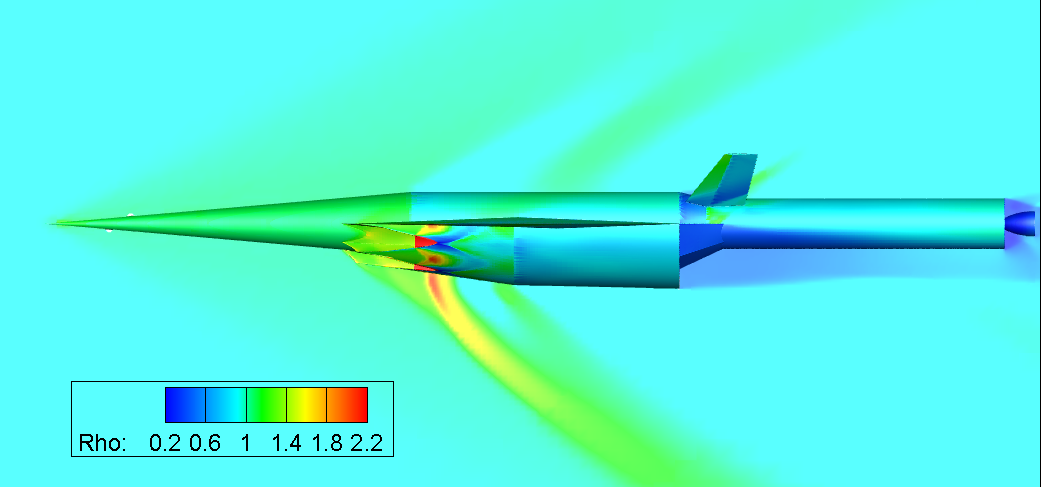
\includegraphics[width=0.6\linewidth]{CARTcontour}
	\caption{Normalised density contours of first stage flight, Mach 2, $-1^\circ$ angle of attack.}
	\label{fig:CARTcontour}
\end{figure}
\begin{figure}[ht]
	\centering
	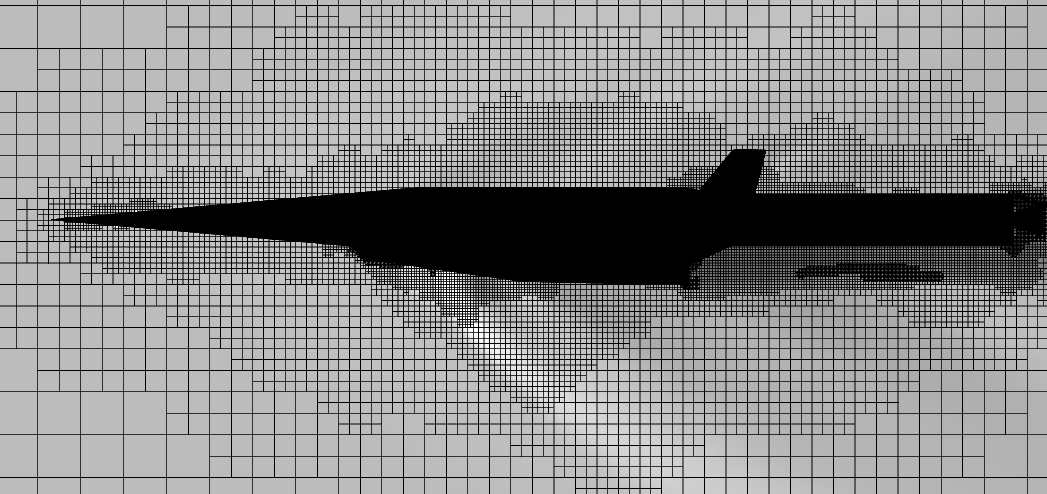
\includegraphics[width=0.6\linewidth]{CARTmesh}
	\caption{Adaptive mesh generated close to vehicle by CART3D for Mach 2, $-1^\circ$ angle of attack flight conditions.}
	\label{fig:CARTmesh}
\end{figure}
\begin{figure}[ht]
	\centering
	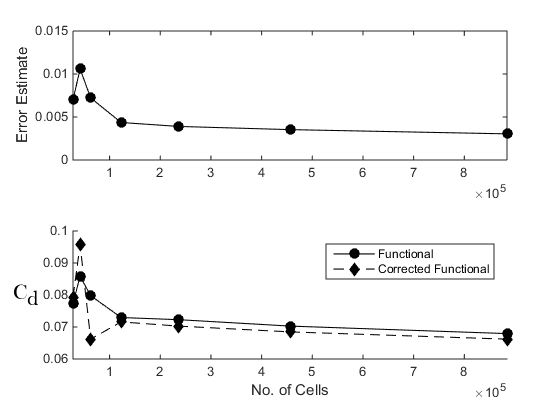
\includegraphics[width=0.4\linewidth]{CART}
	\caption{CART3D verification parameters of error estimate and $C_d$ functional.}
	\label{fig:CART}
\end{figure}
A pressure field for Mach 2, $-1^\circ$ angle of attack calculated using CART3D is shown in Figure \ref{fig:CARTcontour}. Figure \ref{fig:CARTmesh} shows an example of the mesh produced by CART3D. This mesh extends out to 50 body lengths at the far-field boundaries. Figure \ref{fig:CART} examines convergence parameters of the CFD solution; the functional, its adjoint-based correction and error estimate. The functional and corrected functional converge and error estimate decreases steadily as the mesh is refined, indicating mesh convergence.

The aerodynamics of the SPARTAN second stage are simulated using a set of aerodynamic coefficients developed in HYPAERO\DIFdelbegin \DIFdel{\mbox{%DIFAUXCMD
\cite{Jazra2009,Preller2017}}%DIFAUXCMD
}\DIFdelend \DIFaddbegin \DIFadd{\mbox{%DIFAUXCMD
\cite{Jazra2009,Preller2017b}}%DIFAUXCMD
}\DIFaddend . HYPAERO produces aerodynamics for hypersonic vehicles, utilising longitudinal strip theory to solve the surface pressures acting on the vehicle and to provide aerodynamic coefficients over the operating range of Mach numbers, angle of attacks, and flap deflection angles of the vehicle. The flaps are used to trim the SPARTAN throughout its trajectory. 

The aerodynamics of the third stage rocket are determined using a database generated using Missile DATCOM\DIFdelbegin \DIFdel{\mbox{%DIFAUXCMD
\cite{Blake1998}}%DIFAUXCMD
}\DIFdelend \DIFaddbegin \DIFadd{\mbox{%DIFAUXCMD
\cite{Rosema2011}}%DIFAUXCMD
}\DIFaddend , a preliminary design tool for estimating the aerodynamic characteristics of missile configurations. 
To limit the aerodynamic forces on the rocket, \DIFdelbegin \DIFdel{it is assumed that 10$^\circ$ angle of attack at 50kPa produces the maximum normal force allowable by the rocket structure}\DIFdelend \DIFaddbegin \DIFadd{\textcolor{red}{the maximum normal force allowable by the rocket structure is set as the normal force produced by 10$^\circ$ angle of attack at 50kPa flight}}\DIFaddend . The maximum angle of attack of the third stage rocket is \DIFaddbegin \DIFadd{thus }\DIFaddend limited to 10$^\circ$ at 50kPa, and increased with altitude so that the maximum allowable normal force, $F_N$, is kept constant. Thrust vectoring is used to trim the third stage rocket. The maximum thrust vector angle is limited to 8$^\circ$, similar to other small size, pressure-fed rocket engines\cite{Zandbergen}. 

Atmospheric properties are drawn from the U.S. Standard Atmosphere 1976\cite{Administration1976}.  
\subsection{Propulsion}
The first stage Merlin 1-C is modelled by scaling the sea level thrust using the standard rocket thrust equation;

\begin{equation}
T = T_{SL} + (P_{SL}-P_{atm}) A_e,
\end{equation}
where $T_{SL}$ is the sea level thrust, $A_e$ is the exit area of 0.55$m^2$, and $P_{SL}$ and $P_{atm}$ are the atmospheric pressure at sea level and at the current flight altitude respectively. The Merlin 1-C is throttled to a constant 85\% of maximum thrust to enable the rocket to pitch easily, giving a sea level thrust of 472.5kN\cite{Vehicle2008}. The vacuum specific impulse is 304s\cite{Vehicle2008}.

The scramjet engine model used is based on the C-REST database\DIFdelbegin \DIFdel{\mbox{%DIFAUXCMD
\cite{Preller2017}}%DIFAUXCMD
}\DIFdelend \DIFaddbegin \DIFadd{\mbox{%DIFAUXCMD
\cite{Preller2017b}}%DIFAUXCMD
}\DIFaddend , which provides data points of engine performance over inlet conditions within the operational range, at 50kPa dynamic pressure equivalent conditions. This data is interpolated for the given inlet conditions to calculate the exit conditions and the specific impulse produced by the engine. The thrust, $T$, is then obtained by inclusion of the mass flow rate ($\dot{m}$) obtained via the inlet conditions, ie. $T = g_0\dot{m}I_{sp}$.
The C-REST engine is a fixed geometry engine, designed for operability at high Mach numbers\DIFdelbegin \DIFdel{\mbox{%DIFAUXCMD
\cite{Preller2017}}%DIFAUXCMD
}\DIFdelend \DIFaddbegin \DIFadd{\mbox{%DIFAUXCMD
\cite{Preller2017b}}%DIFAUXCMD
}\DIFaddend . At lower Mach numbers, the addition of excessive fuel may cause the engine to choke and unstart, resulting in total loss of thrust\DIFdelbegin \DIFdel{\mbox{%DIFAUXCMD
\cite{Preller2017}}%DIFAUXCMD
}\DIFdelend \DIFaddbegin \DIFadd{\mbox{%DIFAUXCMD
\cite{Preller2017b}}%DIFAUXCMD
}\DIFaddend . To avoid unstart, an equivalence ratio \DIFdelbegin \DIFdel{($\phi$) }\DIFdelend of less than 1 is set at low Mach numbers. 

 The third stage Kestrel engine is modified to provide 50\% increased thrust over the standard Kestrel engine. This has been modelled by increasing the mass flow rate and nozzle throat diameter, although the nozzle exit diameter has not been changed. This results in the nozzle area ratio decreasing from 60\cite{Vehicle2008} to 40, lowering the vacuum efficiency by 2\%\cite{RPE}. The modified third stage Kestrel engine has a vacuum specific impulse of 310.7s\cite{Vehicle2008} and a vacuum thrust of 45.1kN. The thrust is modelled using the standard rocket thrust equation to scale for atmospheric pressure; 
\begin{equation}
T = T_{vac} -P_{atm} \, A_e.
\end{equation}

\subsection{Dynamic Model} \DIFdelbegin %DIFDELCMD < \label{section:dynamics}
%DIFDELCMD < %%%
\DIFdelend \DIFaddbegin \label{subsection:dynamics}
\DIFaddend The drag and lift produced by each stage of the vehicle are calculated using the standard definition of the aerodynamic coefficients:

\begin{equation}
\DIFdelbegin \DIFdel{F_d }\DIFdelend \DIFaddbegin \DIFadd{\textcolor{red}{D} }\DIFaddend = \frac{1}{2} \, \rho \, C_D \, v^2 \, A ,
\end{equation}
\begin{equation}
\DIFdelbegin \DIFdel{F_L }\DIFdelend \DIFaddbegin \DIFadd{\textcolor{red}{L} }\DIFaddend = \frac{1}{2} \, \rho \, C_L \, v^2 \, A .
\end{equation}

The dynamics of all stages are calculated using an geodetic rotational reference frame, written in terms of the radius from centre of Earth $r$, longitude $\xi$, latitude $\phi$, flight path angle $\gamma$, velocity $v$ and heading angle $\zeta$. The equations of motion are\DIFdelbegin \DIFdel{\mbox{%DIFAUXCMD
\cite{Josselyn2002a}}%DIFAUXCMD
}\DIFdelend \DIFaddbegin \DIFadd{\mbox{%DIFAUXCMD
\cite{Josselyn2002}}%DIFAUXCMD
}\DIFaddend :

\begin{equation}
\dot{r} = v \, \sin \gamma
\end{equation}

\begin{equation}
\dot{\xi} = \frac{v \, \cos \gamma \, \cos \zeta}{r \, \cos \phi}
\end{equation}

\begin{equation}
\dot{\phi} = \frac{v\,\cos\gamma\,\sin\zeta}{r}
\end{equation}
\begin{equation}
\dot{\gamma} = \frac{T\,\sin\alpha}{m\,v}+ (\frac{v}{r}-\frac{\mu_E}{r^2 \,v})\,\cos\gamma + \frac{L}{m\,v}
 + \cos\phi[2\,\omega_E\, \cos\zeta + \frac{\omega_E^2\, r}{v}(\cos\phi\,\cos\gamma+\sin\phi\,\sin\gamma\,\sin\zeta)]
 \end{equation}
\begin{equation}
\dot{v} = \frac{T\,\cos\alpha}{m}-\frac{\mu_E}{r^2}\,\sin\gamma - \frac{D}{m}
+ \omega_E^2 r\,\cos\phi(\cos\phi\,\sin\gamma-\sin\phi\,\cos\gamma\,\sin\zeta)
\end{equation}
\begin{equation}
\dot{\zeta} = -\frac{v}{r}\tan\phi\,\cos\gamma\,\cos\zeta +2\,\omega_E\,\cos\phi\,\tan\gamma\,\sin\zeta - \frac{\omega_E^2 r}{v\,\cos\gamma}\,\sin\phi \, \cos\phi\,\cos\zeta-2\omega_E\,\sin\phi 
\end{equation}


\section{Trajectory Optimisation} \label{section:optimisation}

The three stage trajectory of the launch vehicle forms a complex optimisation problem, spanning a large range of velocity and altitude conditions with multiple changes in the vehicle dynamics and propulsion method. In order to simplify the problem, the three stages are calculated separately, and coupled together at the separation points $\textbf{x}_1(t_{1,f})$ (first to second stage) and  $\textbf{x}_2(t_{2,f})$ (second to third stage). Together these problems have the form of a sequential decision making problem, where the global optimal solution can be determined using dynamic programming\cite{Bertsekas2005}. 



\subsection{Trajectory Planning as an Optimal Control Problem}

 The optimal trajectory for each stage is found by determining the control function $\textbf{u}_a(t)$ which minimises the objective function:
\begin{equation} \label{eq:opt}
\min\limits_{\textbf{u}_a} \quad C_a(\textbf{x}_a(t_a),\textbf{u}_a(t_a)) + C_{a\rightarrow  b}(\textbf{x}_a(t_{a,f})),
\end{equation}
where $a$ is the vehicle stage to be optimised and $b$ is the following stage. $ C_a(\textbf{x}_a(t_a),\textbf{u}_a(t_a))$ is a continuous cost function and $C_{{a\rightarrow b}}$ is a terminal cost, dependent on the state variables $\textbf{x}_a(t_{a,f})$ at the end of the stage trajectory. This terminal cost is used in this study to connect the optimal control problem to the next stage, which allows for the overall trajectory to be designed using dynamic programming.
The optimisation of Equation \ref{eq:opt}, subject to the vehicle dynamics, has the form of a Bolza optimisation problem, where an objective function $J(\textbf{x},\textbf{u},t_f)$ is minimised,

\begin{equation} \label{eq:cost}
J(\textbf{x}(t),\textbf{u}(t)) = \underbrace{M[\textbf{x}(t_f)]}_{C_{a\rightarrow  b}(\textbf{x}_a(t_a,{f}))} +   \underbrace{\int_{t_0}^{t_f} P[\textbf{x}(t),\textbf{u}(t)]}_{ C_a(\textbf{x}_a(t_a),\textbf{u}_a(t_a))} dt, \quad t \in [t_0,t_f],
\end{equation}
where $M$ is the terminal cost function and $P$ is the stage cost. The optimisation problem is subject to a set of state dynamics $\dot{\textbf{x}}(t)$, which describe the behaviour of the system over the solution space: 
\begin{equation} \label{eq:state}
\dot{\textbf{x}}_a(t_a) = f[t_a,\textbf{x}_a(t_a),\textbf{u}_a(t_a)].
\end{equation}
These state dynamics correspond to the equations of motion of the vehicle, as defined in Section \DIFdelbegin \DIFdel{\ref{section:dynamics}}\DIFdelend \DIFaddbegin \DIFadd{\ref{subsection:dynamics}}\DIFaddend .
The optimisation problem is constrained by the boundary conditions of the system, at the initial and final time points:
\begin{equation}
\bm{\psi}_0[\textbf{x}_a(t_{a,0}), t_{a,0}] = \textbf{0},
\end{equation}
\begin{equation} \label{eq:2}
\bm{\psi}_f[\textbf{x}_a(t_{a,f}), t_{a,f}] = \textbf{0},
\end{equation}
as well as a set of inequality constraints defining the bounds of the problem:
\begin{eqnarray}
\bm{\lambda}[\textbf{x}_a(t_a),\textbf{u}_a(t_a)] \leq \textbf{0}.
\end{eqnarray}
 These inequality constraints are chosen to span the possible operating \DIFdelbegin \DIFdel{ranges of the first stage and the SPARTAN }\DIFdelend \DIFaddbegin \DIFadd{range of the \textcolor{red}{vehicle} }\DIFaddend to ensure an optimal solution. 
 Solving this Bolza problem in a discrete simulation requires the use of numerical solution methods\DIFdelbegin \DIFdel{for which the pseudospectral method solver DIDO was chosen \mbox{%DIFAUXCMD
\cite{Ross}}%DIFAUXCMD
. 
 }\DIFdelend \DIFaddbegin \DIFadd{. 
 \textcolor{red}{The first and second stage trajectory solutions utilise the pseudospectral method, a form of direct spectral collocation\cite{Fahroo2000,Rao2009}. To perform this optimisation the pseudospectral method solver DIDO was chosen\cite{Ross}}.
}\DIFaddend 


\DIFdelbegin \subsubsection{\DIFdel{The Pseudospectral Method for Optimal Control}}
%DIFAUXCMD
\addtocounter{subsubsection}{-1}%DIFAUXCMD
\DIFdel{The first and second stage trajectory solutions utilise the pseudospectral method, a form of direct spectral collocation \mbox{%DIFAUXCMD
\cite{Fahroo2000}}%DIFAUXCMD
.
The pseudospectral method offers good convergence properties and relatively good computational speed, while not compromising the accuracy of the optimal solution \mbox{%DIFAUXCMD
\cite{Fasano2013}}%DIFAUXCMD
. These properties make the pseudospectral method appropriate for optimising a hypersonic vehicle system. 
The pseudospectral method utilises a spectral collocation method to approximate the optimal control problem as a nonlinear programming problem. The use of the spectral method ensures that higher order terms of the dynamic equations are solved, and facilitates solution with high accuracy, even with relatively few collocation points\mbox{%DIFAUXCMD
\cite{Fahroo1999}}%DIFAUXCMD
. The accuracy and validity of this method has been demonstrated for a variety of aerospace applications \mbox{%DIFAUXCMD
\cite{Bedrossian,Huntington2008,Josselyn2002,Yan2007}}%DIFAUXCMD
. 
}%DIFDELCMD < 

%DIFDELCMD < %%%
\subsubsection{\DIFdel{The Direct Single Shooting Method for Optimal Control}}
%DIFAUXCMD
\addtocounter{subsubsection}{-1}%DIFAUXCMD
%DIFDELCMD < 

%DIFDELCMD < %%%
\DIFdelend The third stage trajectory optimization is performed using the direct single shooting method~\cite{Diehl2006}. The direct single shooting method is selected for the third stage trajectory optimisation due to its ease of initialization, allowing it to automatically solve repeated instances of the problem with different initial conditions. 
The direct single shooting method uses \DIFdelbegin \DIFdel{an SQP }\DIFdelend \DIFaddbegin \DIFadd{\textcolor{red}{an SQP} }\DIFaddend algorithm to directly solve for the optimal time-discretised control history\DIFaddbegin \DIFadd{\textcolor{red}{\cite{Rao2009}}}\DIFaddend .
This control history is optimised subject to the dynamics, cost and constraints of the system, which are evaluated at each iteration using forward simulation.
Due to the strong dependence on the control history, the direct single shooting method is highly sensitive to the initial guess for nonlinear problems, and is mostly suited to solving well-conditioned problems.




\subsection{Optimisation Methodology}
\DIFaddbegin 

\DIFadd{\textcolor{red}{The program LODESTAR (Launch Optimisation and Data Evaluation for Scramjet Trajectory Analysis Research) has been developed to produce an optimal trajectory path for a rocket-scramjet-rocket launch vehicle. LODESTAR provides subroutines which enable the simulation of rocket and scramjet vehicles in 6 degrees of freedom, designed specifically for use within an optimisation routine, including aerodynamic and engine performance calculations as well as trim analysis. LODESTAR also adaptively provides bound and guess inputs to the optimisation routines. In this study LODESTAR utilises a direct single shooting method for the third stage, and DIDO\cite{Ross,Ross2004}, a proprietary pseudospectral method optimisation package, for the first and second stages. DIDO solves the optimisation problem at shifted Legendre-Gauss-Lobatto points, using a spectral algorithm based on an active-set method within SNOPT, an SQP solver\cite{Ross,Gill2002}.} 
}


	 \DIFaddend The three stages are considered as separate optimisation problems, which are coupled at the stage separation points.
	 The first and second stages are coupled by a separation point which is determined by the optimal altitude and \DIFdelbegin \DIFdel{trajectory angle }\DIFdelend \DIFaddbegin \DIFadd{\textcolor{red}{flight path angle} }\DIFaddend for the second stage trajectory, as well as the minimum starting velocity of the scramjet. This separation point is used as an end condition on the first stage optimisation.
	 	 \DIFdelbegin %DIFDELCMD < 

%DIFDELCMD < 	 %%%
\DIFdelend For the minimum pull-up case, the second and third stages are coupled by the end point of the second stage simulation, which is reached when the second stage has expended all of its fuel. The third stage trajectory is optimised for maximum payload from the end of the second stage trajectory.

	 For the maximum payload cases, the second and third stages are coupled \textit{a priori} by running the third stage optimisation repeatedly for different separation altitudes, velocities, and angles and tabulating the results. The terminal cost of payload-to-orbit, for the second stage optimisation, is generated from this table using interpolation. By setting the objective of the third stage optimisation to maximise payload mass, the coupled optimisation of the second stage in turn maximises payload mass over both stages. 
	 The coupling of the stage simulations means that the stage optimisations are performed backwards-in-time to design the complete trajectory; first the third stage is optimised for maximum payload-to-orbit and tabulated over a range of altitudes, velocities and \DIFdelbegin \DIFdel{trajectory angles}\DIFdelend \DIFaddbegin \DIFadd{\textcolor{red}{flight path angle}s}\DIFaddend , then the second stage is optimised for maximum payload-to-orbit, and lastly the first stage is optimised for fuel mass to reach the optimal second stage start point. 

	 
	 
	  \subsubsection{Third Stage Optimisation} \label{section:thirdstage}

	   \begin{figure}[t]
	   	\begin{center}
	   		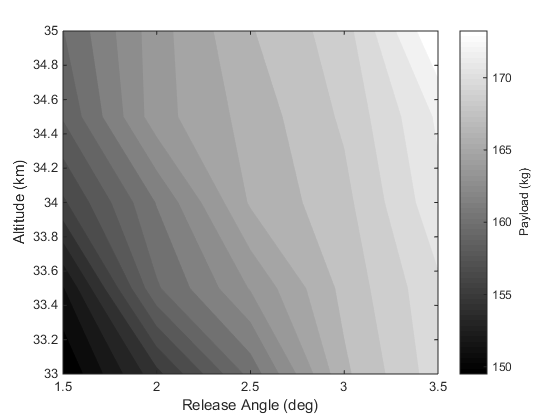
\includegraphics[width=0.6\linewidth]{contours}
	   		\caption{Payload mass results with variation in rocket stage release point for $v$ = 2875m/s, heading angle = 1.78 rad and latitude = -0.136 rad.}
	   		\label{fig:contours}
	   	\end{center}
	   \end{figure}

	  The third stage rocket trajectory is optimised for maximum payload-to-orbit, so that the second stage scramjet and third stage rocket form a Bolza optimisation problem and maximise payload collectively. The cost function is configured to maximise payload at the end of the trajectory:
	  \begin{equation} 
	  \min\limits_{\textbf{u}_3} \quad C_{3\rightarrow LEO}(\textbf{x}_{3}(t_{3,f})) 
	  \end{equation}
	  where
	  \begin{equation}
	  C_{3\rightarrow LEO}(\textbf{x}_{3}(t_{3,f})) = -m_{payload},
	  \end{equation}
	  and $\textbf{x}_{3}(t_{3,f})$ are the tabulated separation conditions of altitude, velocity, and \DIFdelbegin \DIFdel{trajectory angle}\DIFdelend \DIFaddbegin \DIFadd{\textcolor{red}{flight path angle}}\DIFaddend . A direct shooting optimisation is performed with twenty angle of attack node points, interconnected by spline interpolation from separation, $t_{3,0}$, to a variable end time, $t_{AoA,f}$. At this time, the angle of attack is gradually reduced, so that it reaches 0 at the end of burn time, $t_{burn,f}$, also variable.  A constraint is imposed so that the angle of attack must have at least 10 seconds to reduce to 0 at end of burn, ie. $t_{burn,f} - t_{AoA,f} \ge 10$, to allow time for manoeuvring.

	  
	  
	  The payload mass is calculated after the Hohmann transfer to the desired orbit, by taking the remaining fuel to be the effective payload capacity. \DIFdelbegin \DIFdel{Sequential quadratic programming (SQP) }\DIFdelend \DIFaddbegin \DIFadd{\textcolor{red}{SQP} }\DIFaddend is used to find the optimal solution, utilising MATLAB's \textit{fmincon} solver\DIFaddbegin \DIFadd{\mbox{%DIFAUXCMD
\cite{MATLAB}}%DIFAUXCMD
}\DIFaddend .
	    As an example, tabulated optimal payload to orbit results for a 2875m/s third stage release velocity are shown in Figure~\ref{fig:contours}. Payload increases with both altitude and release angle, however it is clear that the potential payload increase due to increasing the separation altitude lessens as release angle increases.  

	
	 
	 	 \subsubsection{Second Stage Optimisation - Constant Dynamic Pressure, Minimum Pull-Up}

	 	 
	 	 The constant dynamic pressure case with minimum pull-up optimises the trajectory to minimise variation from the desired dynamic pressure, with the third stage release angle constrained to 1.5$^\circ$, approximately the minimum release angle necessary to reach orbit. This constraint results in a trajectory with the smallest possible pull-up manoeuvre. 
	 	 The trajectory is configured with a quadratic cost function centred around 50kPa dynamic pressure:
	 	 \begin{equation} 
	 	 \min\limits_{\textbf{u}_2} \quad C_2(\textbf{x}_{2}(t_2),\textbf{u}_{2}(t_2))
	 	 \end{equation}
	 	 where
	 	 \begin{equation}
	 	 C_2(\textbf{x}_{2}(t_2),\textbf{u}_{2}(t_2)) = \int_{t_{2,0}}^{t_{2,f}} \frac{(\textit{\textbf{q}}-50\times 10^3)^2+10^5}{10^5} \, dt
	 	 \end{equation}
	This quadratic function provides a smooth, continuous function to increase solver stability and ensure uniform dynamic pressure. \DIFaddbegin \DIFadd{\textcolor{red}{Scaling and translating constants of $10^5$ are included to normalize the cost function, in order to improve the accuracy and stability of the solution}. }\DIFaddend Second-third stage separation occurs when the scramjet has expended all of its fuel.  The third stage is then optimised for maximum payload from the calculated second-third stage separation point. 

	\DIFaddbegin \DIFadd{\textcolor{red}{In order to ensure an optimal solution, the number of nodes which DIDO uses is manually varied between 96-105, and a solution computed for each node value to ensure a distinct local minima. Ten solutions is observed to provide a sufficient number of node variation, with the solutions converging to similar local minima. The range of node values is chosen to produce accurate solutions, with efficient computation times. The final solution chosen corresponds to the node value which most minimises the cost function, and thus minimises the deviation from the 50kPa dynamic pressure trajectory. }
	 	 }

	 	 \DIFaddend \subsubsection{Second Stage Optimisation - Maximised Payload}
	 For the maximum payload optimisation, the second and third stages are considered using a dynamic programming approach. First, in order to increase the computational efficiency of the optimisation, optimal third stage payloads are tabulated  over a 3 degree grid of separation conditions, $\textbf{x}_2(t_{2,f})$, as described in Section \ref{section:thirdstage}, providing the optimal payload for a range of velocity, altitude and \DIFdelbegin \DIFdel{trajectory angles }\DIFdelend \DIFaddbegin \DIFadd{\textcolor{red}{flight path angle}s }\DIFaddend at separation as shown in Figure \ref{fig:contours}. Then, the interpolated third stage payload is used as the terminal cost $C_{2 \rightarrow 3}(\textbf{x}_2(t_{2,f}))$ for the calculation of the second stage trajectory optimisation, which optimises both the second and third stages by setting the cost function to maximise payload:
	  \begin{equation}
	  \min\limits_{\textbf{u}_2} \quad C_2(\textbf{x}_{2}(t_2),\textbf{u}_{2}(t_2) + C_{2 \rightarrow 3}(\textbf{x}_2 (t_{2,f}))
	  \end{equation}
	  where
	  \begin{equation}
	  C_2(\textbf{x}_{2}(t_2),\textbf{u}_{2}(t_2)) = 0.01\int_{t_{2,0}}^{t_{2,f}}\dot{m}_{fuel} \, dt
	  \end{equation}
	  \begin{equation}
	  C_{2 \rightarrow 3}(\textbf{x}_2(t_{2,f})) = -m_{payload}.
	  \end{equation}
	   $C_{2}(\textbf{x}_{2}(t_2),\textbf{u}_{2}(t_2))$ is included to improve numerical stability and is \DIFdelbegin \DIFdel{chosen }\DIFdelend \DIFaddbegin \DIFadd{\textcolor{red}{weighted by a constant, 0.01, in order} }\DIFaddend to have negligible effect on the resultant trajectory.
	 This problem is solved using the pseudospectral method\cite{Ross2004}.  \DIFaddbegin \DIFadd{\textcolor{red}{As with the constant dynamic pressure case, the number of nodes is manually varied between 96-105, and a solution computed for each node value, converging to similar local minima. The final solution chosen corresponds to the node value which most maximises the payload-to-orbit of the vehicle.} 
	 }\DIFaddend The third stage is optimised for maximum payload from the calculated second-third stage separation point, as a check to ensure that the interpolation has provided an accurate payload-to-orbit result. 

 

\subsubsection{First Stage Optimisation}
After launch, the first stage flies vertically until 100m altitude, when a pitchover is initiated. 
From pitchover, the first stage is optimised for the minimum fuel mass necessary to reach the first-second stage separation conditions, $\textbf{x}_1(t_{1,f})$, of 1520m/s velocity, and altitude and flight path angle determined by the second stage trajectory. 

The separation velocity of 1520m/s corresponds to Mach 5.1 at 50kPa, the minimum operating point of the proposed scramjet\DIFdelbegin \DIFdel{\mbox{%DIFAUXCMD
\cite{Preller2017}}%DIFAUXCMD
}\DIFdelend \DIFaddbegin \DIFadd{\mbox{%DIFAUXCMD
\cite{Preller2017b}}%DIFAUXCMD
}\DIFaddend . Release at the minimum operable point is advantageous, as the scramjet specific impulse increases at low velocities\DIFdelbegin \DIFdel{\mbox{%DIFAUXCMD
\cite{Preller2017}}%DIFAUXCMD
}\DIFdelend \DIFaddbegin \DIFadd{\mbox{%DIFAUXCMD
\cite{Preller2017b}}%DIFAUXCMD
}\DIFaddend .
The altitude and flight path angle at first-second stage separation is defined by the optimised second stage. This approach is used on account of the selected first stage being able to reach the required range of altitudes and flight angles at 1520m/s  with small fuel mass variations. 
Nevertheless\DIFaddbegin \DIFadd{\textcolor{red}{,} }\DIFaddend small variation in fuel mass can have an important effect on the capabilities of the first stage, \DIFdelbegin \DIFdel{determining }\DIFdelend \DIFaddbegin \DIFadd{\textcolor{red}{influencing} }\DIFaddend the velocity achievable at first to second stage separation, as well as the rate at which the rocket is able to pitch, and consequentially, the altitude and flight path angle range of the first stage.
 The \DIFdelbegin \DIFdel{optimum }\DIFdelend \DIFaddbegin \DIFadd{optimal }\DIFaddend (lowest fuel consumption) trajectory for the first stage stack that can reach first-second stage separation condition $\textbf{x}_1(t_{1,f})$ is found by setting a cost function to minimise fuel mass:
\begin{equation}
\min\limits_{\textbf{u}_1} \quad  C_{1 \rightarrow 2}(\textbf{x}_1(t_{1,f}))
\end{equation}
where
\begin{equation}
C_{1 \rightarrow 2}(\textbf{x}_1(t_{1,f})) = m_{fuel}
\end{equation}
and the end point is fixed by the optimal second stage start conditions. The first stage is limited to -5$^\circ$ angle of attack to produce a conservative trajectory solution, within the capabilities of the vehicle. The optimal trajectory is determined using the pseudospectral method. \DIFaddbegin \DIFadd{\textcolor{red}{Three results are obtained by varying the number of nodes in DIDO between 90-92. The computation of three solutions is judged to be sufficient, as the solutions converge to very similar minima, and the fuel mass usage is observed to vary very little. The final result is chosen as the solution which uses the least fuel.}
}\DIFaddend 


\section{Results and Discussion} \label{section:results}
\DIFdelbegin \DIFdel{The program LODESTAR (Launch Optimisation and Data Evaluation for Scramjet Trajectory Analysis Research) was developed to produce an optimal trajectory path for a rocket-scramjet-rocket launch vehicle. LODESTAR utilises DIDO \mbox{%DIFAUXCMD
\cite{Ross,Ross2004}}%DIFAUXCMD
, a proprietary pseudospectral method optimisation package, to optimise a trajectory towards a customisable objective (i.e. constant dynamic pressures or optimal payload mass). 
LODESTAR }\DIFdelend \DIFaddbegin 



\DIFadd{LODESTAR }\DIFaddend is used to investigate the suitability of a pseudospectral method approach to optimisation of scramjet-rocket trajectories and to develop optimal trajectory solutions. The following trajectories are developed: 
\begin{enumerate}
	\item: $q = $ 50kPa fixed SPARTAN trajectory with minimum pull-up \newline$\rightarrow$ Verifies simulation and provides baseline trajectory.
	\item: Trajectory optimised for payload-to-orbit, $q_{max} = $ 50kPa \newline$\rightarrow$ Demonstrates improved performance through coupled trajectory optimisation.
	\item: Trajectory optimised for payload-to-orbit, $q_{max} = $ 45kPa \& $q_{max} = $ 55kPa \newline$\rightarrow$ Comparison of these simulations allows investigation into the effect of $q$ max on payload-to-orbit.
	\item: Trajectory optimised for payload-to-orbit,  $q_{max} = $ 50kpa, 110\% SPARTAN Drag \newline$\rightarrow$ Comparison of optimal trajectories at 100\% and 110\% drag allows investigation of the robustness of the solution with variation in vehicle design. 
\end{enumerate}

Table \ref{table:Summary} details key results for comparison. 


\begin{table}[htb]
	\centering
	\caption{Summary of Simulation Results}
	\small
	\begin{tabular}{l c c c c c}
 & \textbf{1} & \textbf{2} & \textbf{3a} & \textbf{3b} & \textbf{4}  \\ 

 
 
		\hline  \begin{tabular}{@{}c@{}} \textbf{Trajectory Condition}\\  \\  	\end{tabular} &  \begin{tabular}{@{}c@{}}\textbf{$q = $ 50kPa} \\\textbf{$\gamma_{2\rightarrow 3}$= 1.5$^\circ$}\end{tabular}&  \begin{tabular}{@{}c@{}}\textbf{$q \leq $ 50kPa} \\ \textbf{Max $m_{Payload}$}\end{tabular}& \begin{tabular}{@{}c@{}}\textbf{ $q \leq $ 45kPa}  \\ \textbf{Max $m_{Payload}$} \end{tabular} & \begin{tabular}{@{}c@{}}\textbf{$q \leq $ 55kPa} \\\textbf{Max $m_{Payload}$} \end{tabular} &  \begin{tabular}{@{}c@{}}\textbf{$q \leq $ 50kPa} \\ \textbf{Max $m_{Payload}$} \\ \textbf{110\% $C_D$} \end{tabular} \\ 

		
		
		\hline \textbf{Payload to Orbit (kg)}  & \PayloadToOrbitConstq & \PayloadToOrbitFiftykPa & \PayloadToOrbitFortyFivekPa & \PayloadToOrbitFiftyFivekPa & \PayloadToOrbitHighDrag \\ 
		\textbf{Separation Alt, 1$\rightarrow$2 (km)}  & \FirstStageAltConstq & \FirstStageAltFifty & \FirstStageAltFortyFive &  \FirstStageAltFiftyFive &\FirstStageAltHighDrag \\ 
		\textbf{1$^{st}$ Stage Structural Mass Fraction} & \FirstStagesmfConstq & \FirstStagesmfFifty &  \FirstStagesmfFortyFive& \FirstStagesmfFiftyFive  & \FirstStagesmfHighDrag\\ 
		 \textbf{Separation Alt, 2$\rightarrow$3(km)}  & \SeparationAltConstq & \SeparationAltFiftykPa & \SeparationAltFortyFivekPa & \SeparationAltFiftyFivekPa & \SeparationAltHighDrag\\ 
		 \textbf{Separation $v$, 2$\rightarrow$3(m/s)} & \SeparationvConstq  & \SeparationvFiftykPa & \SeparationvFortyFivekPa &  \SeparationvFiftyFivekPa & \SeparationvHighDrag\\ 
		 \textbf{Separation $\gamma$, 2$\rightarrow$3(deg)} & \SeparationAngleConstq& \SeparationAngleFiftykPa &\SeparationAngleFortyFivekPa& \SeparationAngleFiftyFivekPa&\SeparationAngleHighDrag \\ 
		 \textbf{Separation $q$, 2$\rightarrow$3(kPa)} & \SeparationqConstq  &\SeparationqFiftykPa&\SeparationqFortyFivekPa &\SeparationqFiftyFivekPa& \SeparationqHighDrag \\ 
		 \textbf{2$^{nd}$ Stage L/d, 2$\rightarrow$3} & \SeparationLDConstq&\SeparationLDFiftykPa & \SeparationLDFortyFivekPa & \SeparationLDFiftyFivekPa &\SeparationLDHighDrag\\
		 \textbf{2$^{nd}$ Stage Flight Time (s)} & \FlightTimeConstq & \FlightTimeFiftykPa & \FlightTimeFortyFivekPa & \FlightTimeFiftyFivekPa & \FlightTimeHighDrag\\ 
		 %\textbf{3$^{rd}$ Stage Max $q$ (kPa)} &\MaxqConstq  &\MaxqFiftykPa & \MaxqFortyFivekPa &\MaxqFiftyFivekPa & \MaxqHighDrag\\ 
		 \textbf{3$^{rd}$ Stage $t$, $q >$ 20kpa (s)} &\toverConstq &\toverFiftykPa &\toverFortyFivekPa &\toverFiftyFivekPa & \toverHighDrag\\ 

		 
		\hline 
	\end{tabular} 


	\label{table:Summary}
\end{table}


\subsection{First Stage Evaluation - q=50kpa Second Stage Separation}

\begin{figure}[H]
	\centering
	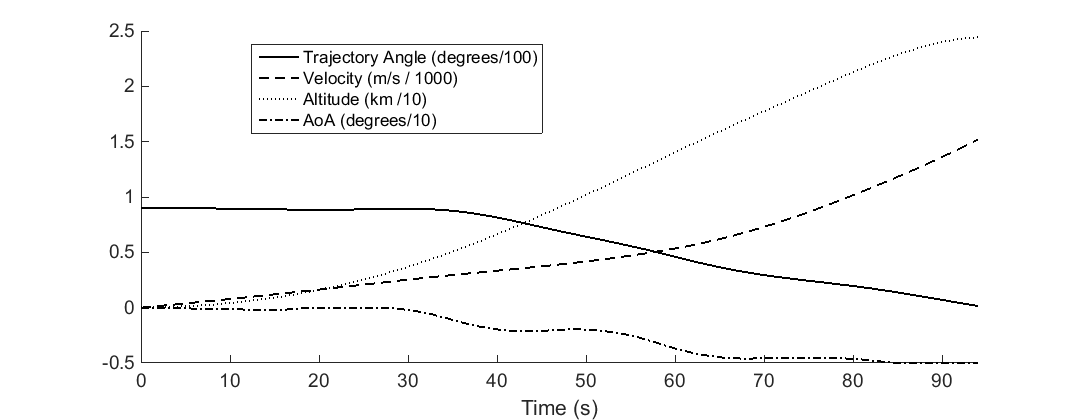
\includegraphics[width=.9\linewidth]{FirstStage}
	\caption{First stage trajectory, optimised for minimum fuel mass and a release point of 50kPa.}
	\label{fig:FirstStage}
\end{figure}

Figure \ref{fig:FirstStage} shows an example first stage trajectory, optimised for minimum mass, with end conditions of 24.4km altitude and 1.56$^\circ$ \DIFdelbegin \DIFdel{trajectory angle}\DIFdelend \DIFaddbegin \DIFadd{\textcolor{red}{flight path angle}}\DIFaddend . These separation conditions correspond to the second stage separation conditions for a 50kpa dynamic pressure trajectory.

The first stage flies a fixed vertical trajectory for 3.74s, after which a pitchover is initiated. 
After pitchover the angle of attack reduces gradually to the minimum of -5$^\circ$, adjusting in stages in order to reach the desired end conditions. 
An altitude of 24.4km is reached after a total flight time of 94.0s, with a total ground distance of 33.3km covered. 
This trajectory shape is very similar for all first stage simulation cases. 



\subsection{Second Stage Evaluation}
\subsubsection{Fixed Dynamic Pressure Trajectory, Minimum Pull-Up} \label{subsection:Fixed}

\begin{figure}[H]
	\centering
	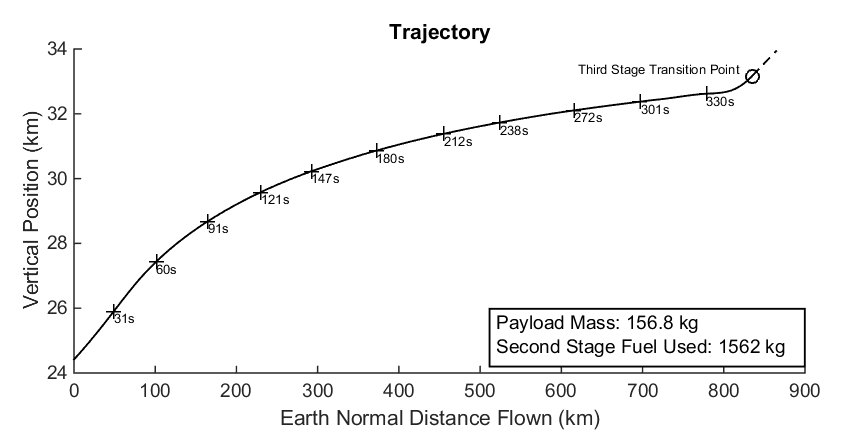
\includegraphics[width=.7\linewidth]{Constq}
	\caption{Trajectory path of the 2$^{nd}$ stage SPARTAN vehicle flying at 50kPa constant dynamic pressure, with 1.5$^\circ$ third stage release angle.}
	\label{fig:constq}
\end{figure}
\begin{figure}[ht]
	\centering	
	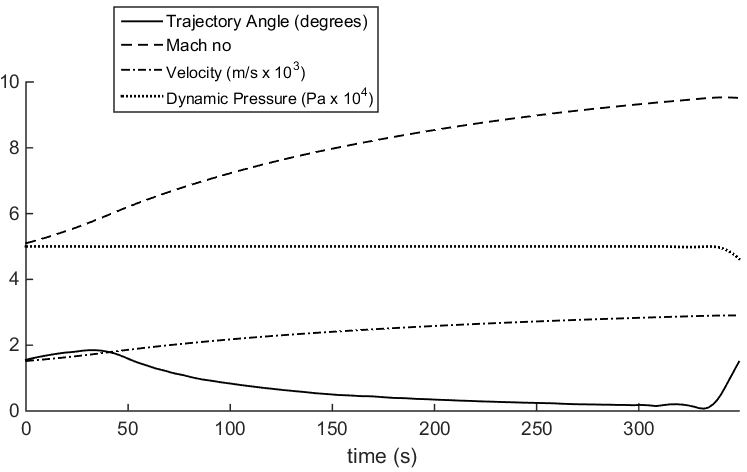
\includegraphics[width=.6\linewidth]{Constq-Aero}
	\caption{Trajectory data for 50kPa constant dynamic pressure trajectory, with 1.5$^\circ$ third stage release angle.}
	\label{fig:constq aero}
\end{figure}
\begin{figure}[ht]
	\centering
	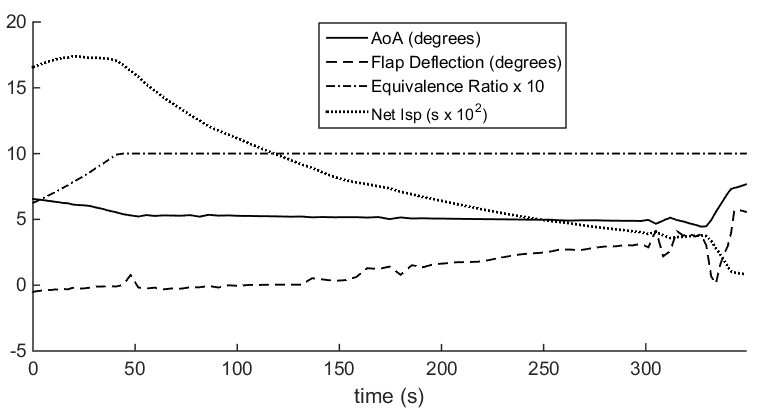
\includegraphics[width=.6\linewidth]{Constq-Vehicle}
	\caption{Vehicle performance data for 50kPa constant dynamic pressure trajectory, with 1.5$^\circ$ third stage release angle. Note: Flap deflection is positive down.}
	\label{fig:constq vehicle}
\end{figure}


A constant dynamic pressure trajectory with a pull-up to 1.5$^\circ$ \DIFdelbegin \DIFdel{trajectory angle }\DIFdelend \DIFaddbegin \DIFadd{\textcolor{red}{flight path angle} }\DIFaddend at third stage release is produced as a baseline for comparison with a payload-optimised trajectory, and to verify that LODESTAR is able to optimise a complex airbreathing trajectory. A pull-up to 1.5$^\circ$ \DIFdelbegin \DIFdel{trajectory angle }\DIFdelend \DIFaddbegin \DIFadd{\textcolor{red}{flight path angle} }\DIFaddend is the minimum necessary for the third stage to reach orbit. At release angles below 1.5$^\circ$, the thrust vector limitations necessary to produce a trimmed trajectory constrain the angle of attack of the third stage so that the rocket does not generate the lift required to exit the atmosphere. This angle of attack limitation, imposed by the maximum thrust vector, necessitates a scramjet-stage pull-up manoeuvre in order for the third stage rocket to operate successfully. 


 The constant dynamic pressure, minimum pull-up trajectory for the SPARTAN stage is shown in Figures \ref{fig:constq}, \ref{fig:constq aero} and \ref{fig:constq vehicle} with key results summarised in Table \ref{table:Summary}. Due to the clear objective of a constant dynamic pressure trajectory, any deviations from the target dynamic pressure are readily apparent, allowing the efficacy of the optimiser to be verified. 
 These results show very close adherence to 50kPa dynamic pressure (maximum 0.29\% deviation) until pull-up at 336.4s. Third stage release occurs at \FlightTimeConstq s at \SeparationAltConstq km altitude. 
 Over the trajectory the Mach no. increases from 5.10 to 9.52 and the velocity from 1520m/s to \SeparationvConstq m/s. The flap deflection shows an overall increase from $-0.53^\circ$ to $5.76^\circ$ over the trajectory.  The net specific impulse (\DIFdelbegin \DIFdel{$I_{sp_{net}} = \frac{T-F_d}{\dot{m}_f g}$}\DIFdelend \DIFaddbegin \DIFadd{$I_{sp_{net}} = \frac{T-\textcolor{red}{D}}{\dot{m}_f g}$}\DIFaddend ) generally decreases over the trajectory, as the efficiency of the scramjet engines decreases. However, at the beginning of the trajectory the equivalence ratio increases as the capture limitations are relaxed with increasing Mach number. This causes the net specific impulse to increase, to a maximum of 1739s, during the first 19.45s flight time. 

Figure \ref{fig:ThirdStageConstQ} shows the corresponding third stage atmospheric exit trajectory after release, evaluated as described in Section \ref{section:rocket}. After atmospheric exit, this trajectory is followed by a Hohmann transfer to a heliosynchronous orbit, resulting in a total payload to orbit of \PayloadToOrbitConstq kg.



\subsubsection{Dynamic Pressure Limited Trajectory} \label{subsection:50kPalimit}



\begin{figure}[ht]
	\centering
	\includegraphics[width=.7\linewidth]{qlimited50kPa}
	\caption{Maximum payload trajectory path of the 2$^{nd}$ stage SPARTAN vehicle when limited to 50kPa dynamic pressure.}
	\label{fig:qlimited}
\end{figure}
\begin{figure}[ht]
	\centering
	\includegraphics[width=.6\linewidth]{qlimited50kPa-aero}
	\caption{Trajectory data for 50kpa dynamic pressure limited trajectory.}
	\label{fig:qlimited aero}
\end{figure}
\begin{figure}[ht]
	\centering
	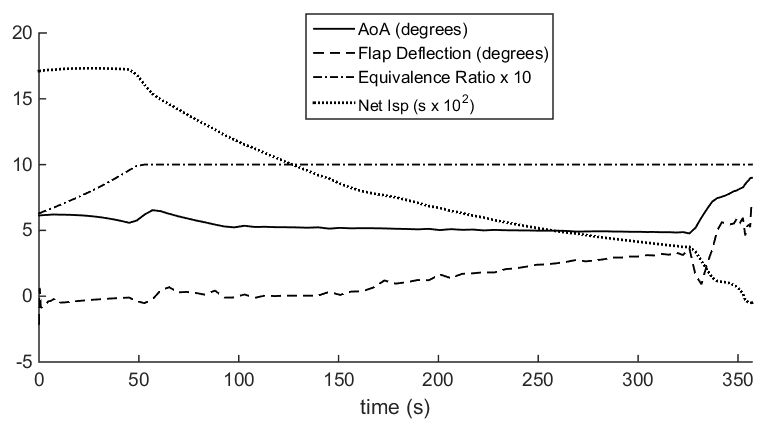
\includegraphics[width=.6\linewidth]{qlimited-Vehicle}
	\caption{Vehicle performance data for 50kpa dynamic pressure limited trajectory. Note: Flap deflection is positive down.}
	\label{fig:qlimited vehicle}
\end{figure}



LODESTAR is configured to optimise the total payload mass to orbit.
A maximum dynamic pressure limit of 50kPa is applied to the optimisation process to allow direct comparison with the constant $q$ trajectory and so that an equivalent vehicle can be used.   

 
The optimal trajectory shape for a $q=$50kPa limited, maximum payload to orbit trajectory is shown in Figures \ref{fig:qlimited}, \ref{fig:qlimited aero} and \ref{fig:qlimited vehicle} with key results summarised in Table \ref{table:Summary}. 
The equivalence ratio of the engine is less than 1 until 52.77s, causing the SPARTAN to fly under 50kPa in this region (to a minimum of 40.8kPa) in order to raise equivalence ratio by flying in a higher temperature region. This increase in equivalence ratio results in a corresponding increase in net specific impulse.
 After the equivalence ratio increases to 1, the trajectory follows a constant dynamic pressure path at 50kPa until 331.7s at which point a pull-up manoeuvre is performed, gaining altitude until rocket stage release at \FlightTimeFiftykPa s flight time. 
 This trajectory is able to deliver \PayloadToOrbitFiftykPa kg of payload to heliocentric orbit, an increase of \PayloadImprovement\ over the constant dynamic pressure result with minimum pull-up. The point at which the pull-up manoeuvre begins is the optimisation result that takes into account the best combination of velocity, altitude and release angle for scramjet stage performance and the release of the rocket stage. This pull-up indicates the region at which increasing altitude and release angle becomes more important than extracting maximum thrust from the scramjet (which is attained at high $q$ and low flight angle at an equivalence ratio of 1).
 Flight in a lower dynamic pressure environment results in less thrust output from the scramjet engines, as well as an increase in angle of attack and flap deflection angle to compensate for the additional lift required. Due to this, less overall acceleration is obtained compared to the constant dynamic pressure result with minimum pull-up. Separation occurs at a velocity of \SeparationvFiftykPa m/s, a decrease of 24m/s. However, at the same time separation altitude increases by 1.32km to \SeparationAltFiftykPa km, resulting in a decrease in separation dynamic pressure to \SeparationqFiftykPa kPa. 

The larger scramjet stage pull-up assists the rocket in manoeuvring to exoatmospheric altitude by increasing the altitude and angle at separation by virtue of the increased L/D ratio and manoeuvrability of the scramjet vehicle. Even a small increase in release angle, to the optimal angle of \SeparationAngleFiftykPa~$^\circ$, significantly reduces the turning that is required by the rocket as evident from comparing Fig \ref{fig:ThirdStageConstQ} and \ref{fig:ThirdStage50kPa}. Further benefits are the reduced time that the rocket must spend in a high dynamic pressure environment, and a decrease in the maximum dynamic pressure that the rocket stage experiences by \qDecrease, as shown in Table \ref{table:Summary}. This allows the structural mass and heat shielding, necessary to achieve exoatmospheric flight, to be decreased, enabling higher payload to orbit. 

 
 Compared to studies considering vehicles with a scramjet-rocket transition within a single stage\cite{Lu1993}\cite{Trefny1999}, the maximum payload to orbit trajectory of the multi-stage system shows a scramjet-rocket transition point at much lower altitudes.
 This lower transition point is a consequence of the stage separation creating an energy trade-off, which does not occur in a single stage vehicle. Single-stage vehicles must necessarily transport all components to exoatmosphere, and so utilise the scramjet engines until higher altitude to take advantage of their high efficiency. A multi-stage vehicle is able to separate the scramjet stage. 
This separation occurs when the performance benefits provided by the superior aerodynamics and engine efficiency of the scramjet stage are offset by the energy required to lift the extra mass to higher altitude. The beneficial ability
to separate the scramjet stage results in a lower altitude scramjet-rocket transition point, when compared to single
stage vehicle designs.

\subsubsection{Dynamic Pressure Sensitivity}\label{subsection:qvariation}
\begin{figure}[ht]
	\centering
	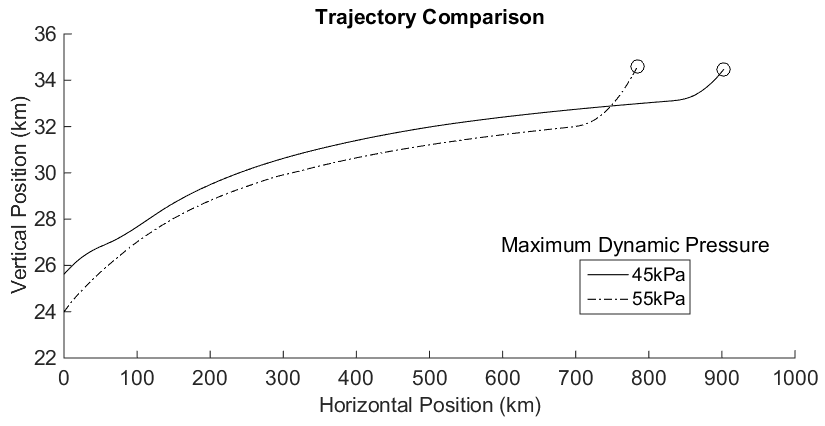
\includegraphics[width=.7\linewidth]{Multipleq}
	\caption{Comparison of 45kPa / 55kpa dynamic pressure limited trajectory paths for maximum payload to orbit.}
	\label{fig:multipleq}
\end{figure}
\begin{figure}[ht]
	\centering

	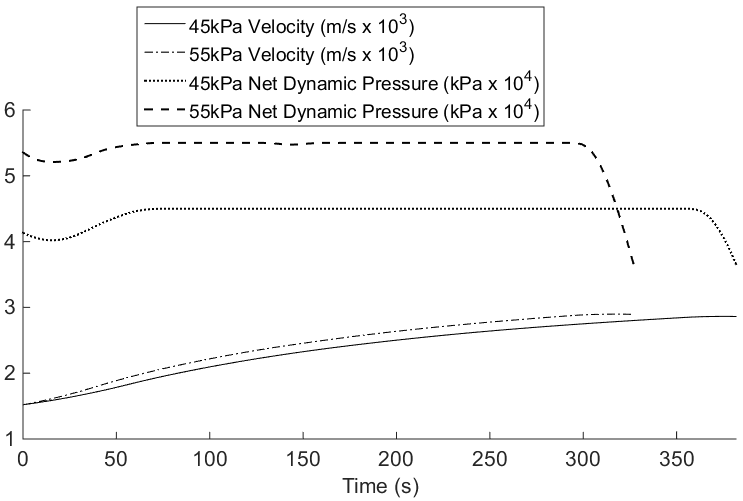
\includegraphics[width=.6\linewidth]{MultipleqAero}
	\caption{Comparison of trajectory data for 45kPa / 55kpa dynamic pressure limited trajectories.}
	\label{fig:multipleq aero}
\end{figure}
\begin{figure}[ht]
	\centering
	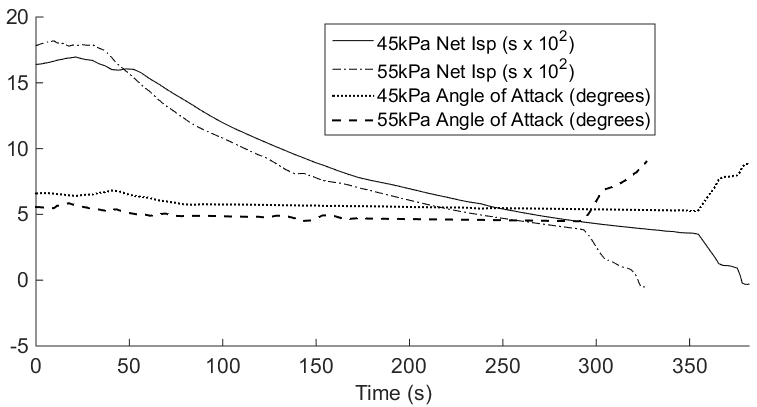
\includegraphics[width=.6\linewidth]{Multipleq-Vehicle}
	\caption{Comparison of vehicle performance data for 45kPa / 55kpa dynamic pressure limited trajectories.}
	\label{fig:multipleq vehicle}
\end{figure}
To investigate the sensitivity of the vehicle to changes in $q_{max}$, the maximum dynamic pressure is varied to 45kPa and 55kPa and the flight trajectory optimised, with results shown in Figures \ref{fig:multipleq}, \ref{fig:multipleq aero} and \ref{fig:multipleq vehicle} and summarised in Table \ref{table:Summary}.
The $\pm10\%$ variation in maximum dynamic pressure has very little effect on the payload mass delivered to heliocentric orbit.  Varying the maximum dynamic pressure by $\pm$5kPa from 50kPa causes a variation of only  \qVariationPluskg (\qVariationPlus) or \qVariationMinuskg (\qVariationMinus) in payload to orbit.  
 Separation altitudes of \SeparationAltFortyFivekPa km and \SeparationAltFiftyFivekPa km are reached  for 45kPa and 55kPa limited cases respectively, with separation velocities of \SeparationvFortyFivekPa m/s and \SeparationvFiftyFivekPa m/s. The 45kPa limited case flies for \FlightTimeFortyFivekPa s, significantly longer than the 55kPa case which flies for \FlightTimeFiftyFivekPa s.
 Both trajectories pull-up to similar altitudes, with relatively small variation in separation velocity \vVariationMinus m/s or \vVariationPlus m/s).
  This small variation in velocity is despite the increase in air density and decrease in angle of attack required for flight at 55kPa dynamic pressure, both of which increase the mass flow into the engine. Although the thrust output of the REST engines increases with dynamic pressure, so does the drag on the vehicle, and the net increase in performance is small. 


Only \DIFaddbegin \DIFadd{\textcolor{red}{a} }\DIFaddend small variation in optimal payload mass is observed, without modification of vehicle design to account for the dynamic pressure limit. This indicates that designing and operating a vehicle at lower dynamic pressures may be preferable. Flying at a lower maximum dynamic pressure allows reduction of the structural weight and heat shielding of the vehicle. However, as the 45kPa limited case has a higher first-second stage separation altitude, a larger first stage fuel mass is required, though this increase in fuel mass is small. Between \FirstStageAltFortyFive km  and \FirstStageAltFiftyFive km (45kPa and 55kPa optimal start points) there is only a \FirstStagemincrease \% variation in the fuel mass required. This small variation in first stage fuel consumption would easily be offset by a decrease in second stage structural mass. 


\subsubsection{Drag Sensitivity Analysis}\label{subsection:dragvariation}
\begin{figure}[ht]
	\centering
	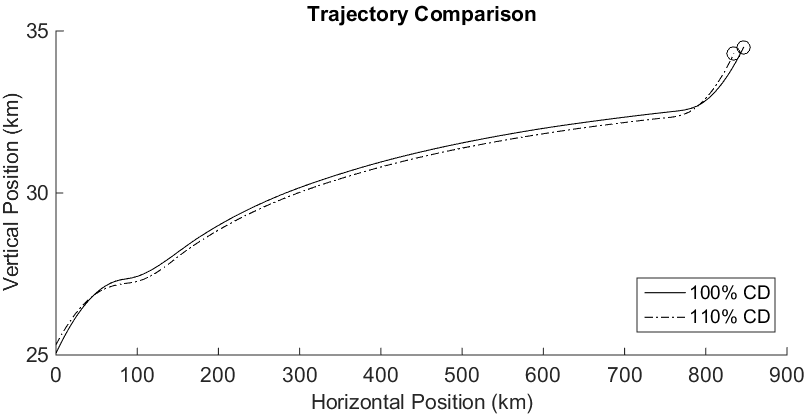
\includegraphics[width=.7\linewidth]{DragComparisonTraj}
	\caption{Comparison of trajectory paths for 100\% and 110\% drag cases for a 50kPa dynamic pressure limited maximum payload trajectory.}
	\label{fig:DragCompTraj}
\end{figure}

\begin{figure}[ht]
	\centering
	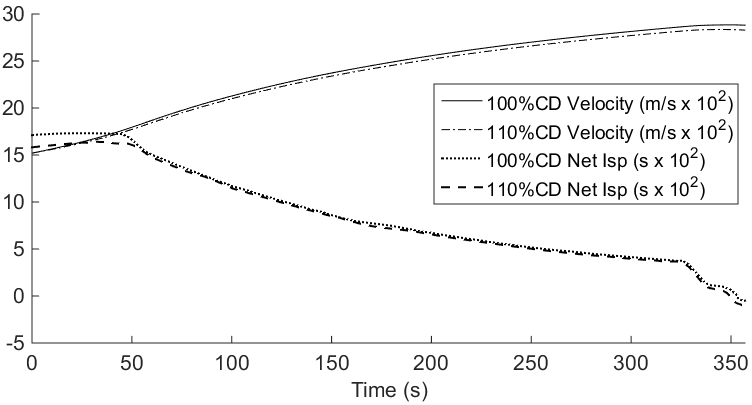
\includegraphics[width=.6\linewidth]{DragComparisonOther}
	\caption{Comparison of $v$ and $I_{sp_{net}}$ for 100\% and 110\% drag cases for a 50kPa dynamic pressure limited maximum payload trajectory.}
	\label{fig:DragCompOther}
\end{figure}

To investigate the effect of vehicle design and uncertainty in aerodynamic performance on the optimal trajectory the drag on the vehicle is increased by 10\%, and an optimised trajectory calculated with dynamic pressure limited to 50kpa. Selected results are compared to the 100\% drag result in Figures \ref{fig:DragCompTraj} and \ref{fig:DragCompOther}. 
These results show that when drag is increased (ie. L/\DIFdelbegin \DIFdel{d }\DIFdelend \DIFaddbegin \DIFadd{\textcolor{red}{D} }\DIFaddend is decreased) the optimal trajectory shape is similar to the base-line case, though the high drag second stage follows a slightly slower and hence lower flight path, with a lower stage transition point. The similar flight path shape of the high drag case suggests that sacrificing velocity to increase separation altitude in a pull-up manoeuvre is optimal for multiple vehicle designs. Although the lower transition point indicates that the rocket is favoured at an earlier point in the climb manoeuvre, due to the decreased aerodynamic efficiency of the scramjet vehicle. 
The net result is  a lower payload-to-orbit of \PayloadToOrbitHighDrag kg (a decrease of 4.8\%). 



 
\subsection{Third Stage Evaluation}

Third stage trajectories for release angles of \SeparationAngleConstq $^\circ$ and \SeparationAngleFiftykPa $^\circ$ are shown in Figures \ref{fig:ThirdStageConstQ} and \ref{fig:ThirdStage50kPa}. 
These trajectories correspond to third stage release points at the end of a constant dynamic pressure trajectory with minimum pull-up (as shown in Section \ref{subsection:Fixed}) and an optimised 50kPa limited trajectory  (as shown in Section \ref{subsection:50kPalimit}). 
These third stage trajectories show a pull-up to high altitude before the circularisation burn is performed. 

The third stage released at 1.5$^\circ$, shown in Figure \ref{fig:ThirdStageConstQ}, is limited by the maximum thrust vector angle for the first 47s of flight. This places significant limitations on the maximum allowable angle of attack. This angle of attack limitation reduces the lift of the rocket, causing it to spend a large amount of time at low altitude, in a high drag environment. The angle of attack increases gradually to a maximum of 17.6$^\circ$ at 66s before decreasing until burnout at 140s. 

The release of the third stage rocket from an optimised scramjet trajectory is shown in Figure \ref{fig:ThirdStage50kPa}. Release at a higher, more optimal angle, mitigates the effects of the thrust vector angle limitation, so that the thrust vector limit is only reached during the first 10s flight time. After this, the angle of attack is limited by the maximum allowable normal force rather than the thrust vector limit, resulting in a higher maximum angle of attack. The rocket increases \DIFdelbegin \DIFdel{trajectory angle }\DIFdelend \DIFaddbegin \DIFadd{\textcolor{red}{flight path angle} }\DIFaddend and gains altitude rapidly, resulting in less time spent in a high drag environment, and a larger payload to orbit.  The angle of attack is increased gradually to 18.14$^\circ$ at 48s, before decreasing until burnout at 138s.

\begin{figure}[H]
	\centering
	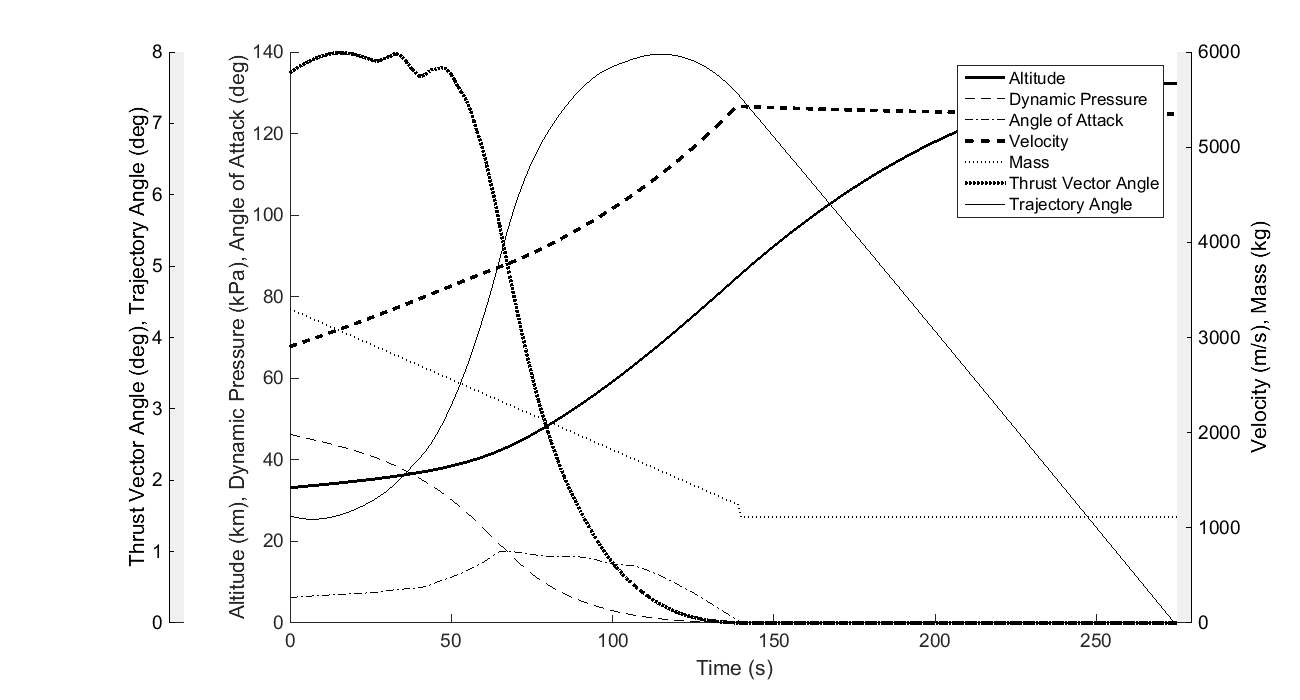
\includegraphics[width=0.8\linewidth]{ThirdStageConstQ}
	\caption{Third stage rocket trajectory simulated from the end of the 50kPa constant dynamic pressure SPARTAN trajectory, released at an angle of \SeparationAngleConstq $^\circ$, velocity of \SeparationvConstq m/s, and altitude of \SeparationAltConstq km.}
	\label{fig:ThirdStageConstQ}
\end{figure}
\begin{figure}[H]

	\centering
	\includegraphics[width=0.8\linewidth]{ThirdStage50kpaConstrained}
	\caption{Third stage rocket trajectory simulated from the end of the 50kPa dynamic pressure limited maximum payload SPARTAN trajectory, released at an angle of \SeparationAngleFiftykPa $^\circ$, velocity of \SeparationvFiftykPa m/s, and altitude of \SeparationAltFiftykPa km.}
	\label{fig:ThirdStage50kPa}
\end{figure}

\section{Conclusions}


In this paper an optimal control program, LODESTAR, is used to design the trajectory of a rocket-scramjet-rocket multi-stage system. This system consists of a rocket-powered first stage, modelled on a scaled down LOX-kerosene SpaceX Falcon-1e; the SPARTAN, a scramjet accelerator being developed at the University of Queensland; and a LOX-kerosene rocket-powered third stage based on the SpaceX Kestrel engine. Applied to full trajectory optimisation, LODESTAR is able to generate optimised trajectories that increased the payload to orbit of the multi-stage system.

   When flying at a constant 50kPa dynamic pressure, results indicate that a scramjet-stage pull-up, to a minimum of \SeparationAngleConstq $^\circ$ \DIFdelbegin \DIFdel{trajectory angle}\DIFdelend \DIFaddbegin \DIFadd{\textcolor{red}{flight path angle}}\DIFaddend , is necessary in order for the third stage rocket to reach orbit successfully. Trajectory optimisation for maximum payload indicates that the optimal scramjet flight path for a system transitioning between separate airbreathing and rocket-powered stages is to fly at lower than maximum dynamic pressure while equivalence ratio is less than 1, followed by constant dynamic pressure flight at maximum dynamic pressure, and finally a pull-up manoeuvre. The optimal pull-up manoeuvre trades off velocity (a decrease of 24m/s) for altitude (an increase of 1.32km) and improved \DIFdelbegin \DIFdel{trajectory angle }\DIFdelend \DIFaddbegin \DIFadd{\textcolor{red}{flight path angle} }\DIFaddend (an increase of 1.41$^\circ$), when compared to the minimum pull-up case. The optimal flight path increases payload mass to heliocentric orbit by 13.1kg (\PayloadImprovement) compared to a constant dynamic pressure trajectory with minimum necessary pull-up. The larger pull up manoeuvre in the payload-optimised trajectory also reduces third stage dynamic pressure to \SeparationqFiftykPa kPa, a decrease of \qDecrease\ compared to a trajectory with minimum pull-up. This decrease in maximum dynamic pressure decreases the stress experienced by the rocket stage proportionally, as well as decreasing the heat flux into the rocket, both of which lead to significant benefits for the design of the rocket stage (which are not taken into account in this study). A decrease in structural stress allows for less internal reinforcement, and a decrease in heat flux allows for reduction of the heat shield size, potentially resulting in further increases in payload mass.


As part of a dynamic pressure sensitivity evaluation, the maximum dynamic pressure limit of the SPARTAN vehicle is varied by $\pm$5kPa. This produces only a \qVariationPlus\ and \qVariationMinus \space variation on the payload mass delivered to orbit. This small variation in payload-to-orbit indicates that a scramjet-powered stage designed for operation at lower dynamic pressure may be advantageous.
If efficient, low dynamic pressure scramjet engines are available, operating at lower dynamic pressure enables lighter vehicles due to reduced structural and thermal loads. This reduction in mass potentially leads to further performance improvements and operational benefits including increased payload to orbit and extended range.

 To investigate the effect of changes in second stage vehicle properties, the drag of the scramjet is increased by 10\% and the optimal trajectory evaluated. This resulted in a pull-up manoeuvre with a lower second-third stage transition point when compared to the original result. This variation in the optimal trajectory is minor, indicating that the presented trajectory shape is robust with respect to changes in vehicle design and, by extension, changes in engine performance or vehicle aerodynamics. Overall this work provides new insight into the preferred operating ranges for scramjet vehicles incorporated in multi-stage to orbit systems\DIFaddbegin \DIFadd{.
}

 
\section*{\DIFadd{Funding Information}}
\DIFadd{This research was supported in part by an Australian Government Research Training Program (RTP) Scholarship}\DIFaddend .

\section*{Acknowledgments}

The authors would like to thank Dawid Preller for his work on the SPARTAN vehicle which is integral to this study, and Joseph Chai for providing the CAD model of the SPARTAN.

\footnotesize

%\bibliographystyle{AIAA}
\bibliography{library}

\end{document}


